% Options for packages loaded elsewhere
\PassOptionsToPackage{unicode}{hyperref}
\PassOptionsToPackage{hyphens}{url}
%
\documentclass[
  ignorenonframetext,
]{beamer}
\title{What are models for and can we use them more effectively?}
\author{Kim Cuddington (\url{https://ecotheory.ca})}
\date{16/05/2022}

\usepackage{pgfpages}
\setbeamertemplate{caption}[numbered]
\setbeamertemplate{caption label separator}{: }
\setbeamercolor{caption name}{fg=normal text.fg}
\beamertemplatenavigationsymbolsempty
% Prevent slide breaks in the middle of a paragraph
\widowpenalties 1 10000
\raggedbottom
\setbeamertemplate{part page}{
  \centering
  \begin{beamercolorbox}[sep=16pt,center]{part title}
    \usebeamerfont{part title}\insertpart\par
  \end{beamercolorbox}
}
\setbeamertemplate{section page}{
  \centering
  \begin{beamercolorbox}[sep=12pt,center]{part title}
    \usebeamerfont{section title}\insertsection\par
  \end{beamercolorbox}
}
\setbeamertemplate{subsection page}{
  \centering
  \begin{beamercolorbox}[sep=8pt,center]{part title}
    \usebeamerfont{subsection title}\insertsubsection\par
  \end{beamercolorbox}
}
\AtBeginPart{
  \frame{\partpage}
}
\AtBeginSection{
  \ifbibliography
  \else
    \frame{\sectionpage}
  \fi
}
\AtBeginSubsection{
  \frame{\subsectionpage}
}
\usepackage{amsmath,amssymb}
\usepackage{lmodern}
\usepackage{iftex}
\ifPDFTeX
  \usepackage[T1]{fontenc}
  \usepackage[utf8]{inputenc}
  \usepackage{textcomp} % provide euro and other symbols
\else % if luatex or xetex
  \usepackage{unicode-math}
  \defaultfontfeatures{Scale=MatchLowercase}
  \defaultfontfeatures[\rmfamily]{Ligatures=TeX,Scale=1}
\fi
% Use upquote if available, for straight quotes in verbatim environments
\IfFileExists{upquote.sty}{\usepackage{upquote}}{}
\IfFileExists{microtype.sty}{% use microtype if available
  \usepackage[]{microtype}
  \UseMicrotypeSet[protrusion]{basicmath} % disable protrusion for tt fonts
}{}
\makeatletter
\@ifundefined{KOMAClassName}{% if non-KOMA class
  \IfFileExists{parskip.sty}{%
    \usepackage{parskip}
  }{% else
    \setlength{\parindent}{0pt}
    \setlength{\parskip}{6pt plus 2pt minus 1pt}}
}{% if KOMA class
  \KOMAoptions{parskip=half}}
\makeatother
\usepackage{xcolor}
\IfFileExists{xurl.sty}{\usepackage{xurl}}{} % add URL line breaks if available
\IfFileExists{bookmark.sty}{\usepackage{bookmark}}{\usepackage{hyperref}}
\hypersetup{
  pdftitle={What are models for and  can we use them more effectively?},
  pdfauthor={Kim Cuddington (https://ecotheory.ca)},
  hidelinks,
  pdfcreator={LaTeX via pandoc}}
\urlstyle{same} % disable monospaced font for URLs
\newif\ifbibliography
\usepackage{graphicx}
\makeatletter
\def\maxwidth{\ifdim\Gin@nat@width>\linewidth\linewidth\else\Gin@nat@width\fi}
\def\maxheight{\ifdim\Gin@nat@height>\textheight\textheight\else\Gin@nat@height\fi}
\makeatother
% Scale images if necessary, so that they will not overflow the page
% margins by default, and it is still possible to overwrite the defaults
% using explicit options in \includegraphics[width, height, ...]{}
\setkeys{Gin}{width=\maxwidth,height=\maxheight,keepaspectratio}
% Set default figure placement to htbp
\makeatletter
\def\fps@figure{htbp}
\makeatother
\setlength{\emergencystretch}{3em} % prevent overfull lines
\providecommand{\tightlist}{%
  \setlength{\itemsep}{0pt}\setlength{\parskip}{0pt}}
\setcounter{secnumdepth}{-\maxdimen} % remove section numbering
\ifLuaTeX
  \usepackage{selnolig}  % disable illegal ligatures
\fi

\begin{document}
\frame{\titlepage}

\begin{frame}
\begin{block}{Co-authors}
\protect\hypertarget{co-authors}{}
Warren Currie (https:) Debora Laura
\end{block}

\begin{block}{Plan}
\protect\hypertarget{plan}{}
\begin{itemize}
\tightlist
\item
  Epistemology: a brief and idiosyncratic overview
\item
  Mechanism and novel conditions
\item
  How can we use models more effectively

  \begin{itemize}
  \tightlist
  \item
    machine learning models: big data and mechanism (Maxent)
  \item
    mathematical models: mining models for data collection directions?
    (Laubiemier)
  \item
    statistical models: using mathematical models to understand
    alternative mechanisms (Quinte)
  \end{itemize}
\end{itemize}
\end{block}
\end{frame}

\begin{frame}{Epistemology: How do we gain knowledge}
\protect\hypertarget{epistemology-how-do-we-gain-knowledge}{}
\note{This is my \emph{note}.

\begin{itemize}
\tightlist
\item
  It can contain markdown
\item
  like this list
\end{itemize}}

\begin{block}{Gaining knowledge in science}
\protect\hypertarget{gaining-knowledge-in-science}{}
\begin{itemize}
\tightlist
\item
  reality
\item
  data: a biased subset of reality
\item
  opinion: what we believe about reality
\end{itemize}

{\(\rightarrow\)Science}: an attitude linking belief and data, whereby
we do not, at least in principle, maintain beliefs that are not
supported by data
\end{block}

\begin{block}{Scientific Theory}
\protect\hypertarget{scientific-theory}{}
\begin{itemize}
\item
  We may refer to beliefs supported by data, or which at least do not
  always contradict data, as \textbf{theories}
\item
  We will like theories to have a few other properties such as:

  \begin{itemize}
  \tightlist
  \item
    logical consistency
  \item
    coherence with other scientific theories
  \end{itemize}
\end{itemize}
\end{block}

\begin{block}{Where do models fit in?}
\protect\hypertarget{where-do-models-fit-in}{}
\begin{itemize}
\item
  Model: a representation of reality
\item
  A structure that:

  \begin{itemize}
  \tightlist
  \item
    embodies some of our beliefs about reality e.g., predators
    negatively impact prey populations \(\frac{dN}{dt}=f(N)-g(N,P)\)
  \item
    mimics some aspect of data e.g., linear regression
    \(y_i=\beta_0+\beta_1x_i+\epsilon\)
  \item
    combines these two components (e.g., makes a statement about the
    expected pattern of data in light of theory)predator consumption
    rate can be described as a type II functional response:
    \(\frac{g(N,P)}{P}=\frac{aN}{N+N_0}\)
  \end{itemize}
\end{itemize}
\end{block}

\begin{block}{Types of models}
\protect\hypertarget{types-of-models}{}
\begin{itemize}
\item
  conceptual (e.g., a statement)
\item
  physical (e.g., lab experiment)
\item
  mathematical (e.g., ODE)
\item
  data-driven (e.g., regression)
\item
  computational (e.g., IBM)
\end{itemize}

``predators can positively impact prey''

\begin{figure}

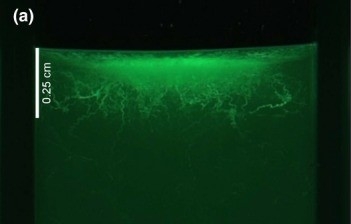
\includegraphics[width=0.35\linewidth]{laurawormscropped} \hfill{}

\caption{Bell & Cuddington 2018}\label{fig:pressure}
\end{figure}

\(\frac{dN}{dt}=f(N,E)+g(N,P,E)\)

\(E(y_i)=β_0+f(x_i)+\epsilon\)

\begin{figure}


\includegraphics[width=0.25\linewidth]{euclidIBM} \hfill{}

\caption{Cuddington & Yodzis 1999}\label{fig:p2}
\end{figure}
\end{block}

\begin{block}{Characteristics of models}
\protect\hypertarget{characteristics-of-models}{}
\begin{itemize}
\tightlist
\item
  trade off precision, generality and realism (Levins 1966).
\item
  is not possible to include all details of a system and still have a
  useful tool (e.g., a one-to-one scale map of a city may include all
  details but is useless as a guide to finding your hotel)
\end{itemize}

``We actually made a map of the country, on the scale of a mile to the
mile!''``Have you used it much?'' I enquired.``It has never been spread
out, yet,'' said Mein Herr, ``the farmers objected: they said it would
cover the whole country, and shut out the sunlight! So we now use the
country itself, as its own map, and I assure you it does nearly as well.
Lewis Carroll - The Complete Illustrated Works. Gramercy Books, New York
(1982)

\begin{itemize}
\tightlist
\item
  therefore, models are always false in some aspects of their
  representation theory or data
\end{itemize}
\end{block}

\begin{block}{Complexity is not necessarily better}
\protect\hypertarget{complexity-is-not-necessarily-better}{}
\begin{itemize}
\tightlist
\item
  think about the map example: complexity is not necessarily helpful for
  explanation
\item
  complexity is not necessarily helpful for prediction either
\end{itemize}

\begin{itemize}
\tightlist
\item
  complex models are prone overfitting
\end{itemize}

``With four parameters I can fit an elephant, and with five I can make
him wiggle his trunk.'' John von Neumann

\begin{itemize}
\tightlist
\item
  don't be impressed impressed when a complex model fits a data set
  well. With enough parameters, you can fit any data set
\end{itemize}

\begin{figure}

{\centering 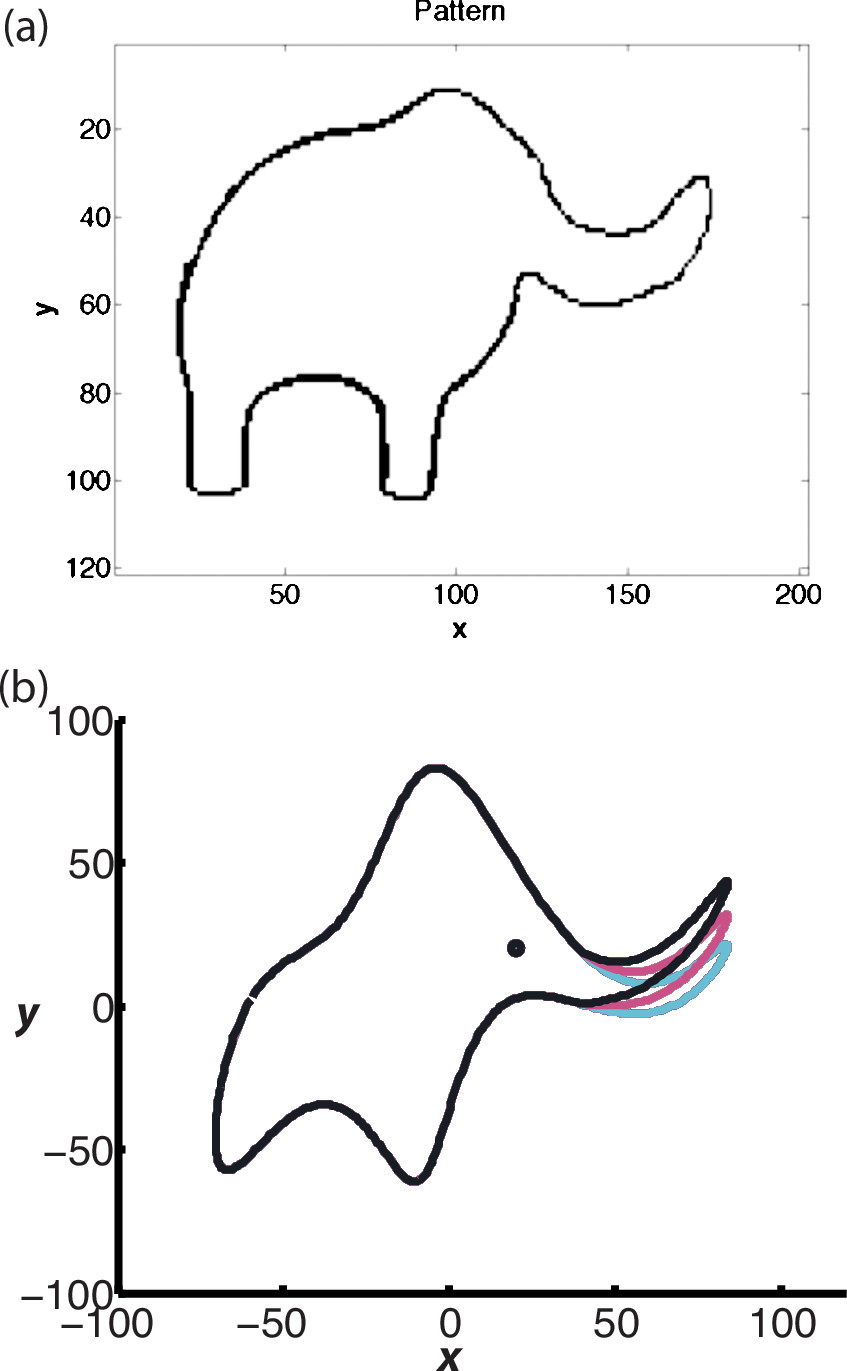
\includegraphics[width=0.65\linewidth]{elephant} 

}

\caption{Mayer et al. 2010}\label{fig:p4}
\end{figure}
\end{block}

\begin{block}{Overfitting}
\protect\hypertarget{overfitting}{}
\begin{itemize}
\tightlist
\item
  but it fits right??
\item
  No not really Overfitting occurs when data-driven model tries to cover
  all the data points in the dataset
\item
  as a result, the model starts caching noise and inaccurate values
  present in the dataset, and all these factors reduce the efficiency
  and accuracy of the model
\end{itemize}

\begin{figure}

{\centering 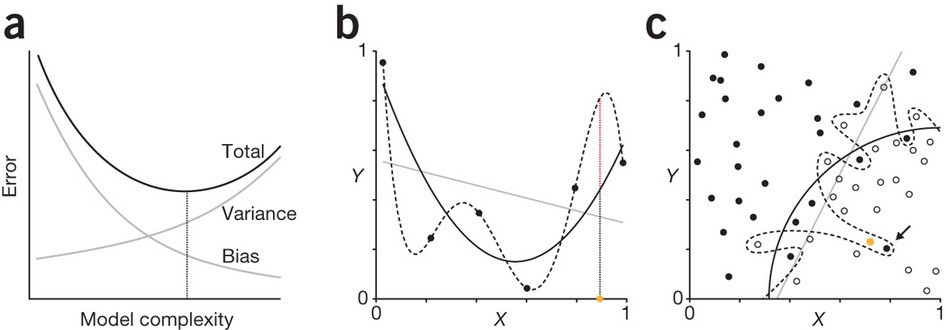
\includegraphics[width=0.8\linewidth]{overfit} 

}

\caption{Lever et al. 2016}\label{fig:p3}
\end{figure}

{\(\rightarrow\)}Complex models \(\neq\) accurate prediction
\end{block}

\begin{block}{Simplicity is not necessarily better}
\protect\hypertarget{simplicity-is-not-necessarily-better}{}
\begin{itemize}
\tightlist
\item
  Simple models \(\neq\) reality/truth (fish stocks environmental
  variation?)
\end{itemize}

{\(\rightarrow\)} Model \(\neq\) reality
\end{block}

\begin{block}{Characteristics of models}
\protect\hypertarget{characteristics-of-models-1}{}
{\(\rightarrow\)} Theory \(\neq\) Model \(\neq\) Reality
\end{block}

\begin{block}{Why do we need models then?}
\protect\hypertarget{why-do-we-need-models-then}{}
\begin{enumerate}
\tightlist
\item
  Explanation
\item
  Prediction
\end{enumerate}

while we attempt to make do without it, both of these functions require
mechanism
\end{block}

\begin{block}{All models can include phenomological or mechanistic
components or both}
\protect\hypertarget{all-models-can-include-phenomological-or-mechanistic-components-or-both}{}
Valle et al.~(2009) found that alternate modelingassumptions in the
forest stand simulation modelSYMFOR can account for 66--97\%of the
variancein predicted stand dynamics. While the authorswere able to
complete this comparison ofdiffering models formulations for SYMFOR,
theynote that it may be very difficult to do the samefor exceedingly
complex models.
\end{block}
\end{frame}

\begin{frame}{The role of mechanism in modelling}
\protect\hypertarget{the-role-of-mechanism-in-modelling}{}
\begin{block}{Data-driven models by themselves, are generally not
mechanistic }
\protect\hypertarget{data-driven-models-by-themselves-are-generally-not-mechanistic}{}
\begin{itemize}
\tightlist
\item
  I'm including here standard statistical models (both frequentist and
  Bayesian), as well as machine learning models
\item
  we might look for a relationship
\end{itemize}

Because these models arebased on causal mechanisms rather than
correla-tion, our confidence in extrapolating beyondknown data is
enhanced. Of course, there isalways uncertainty about how an
ecologicalprocess will interact with novel global changeconditions.

However, underconditions of global change, models based on thepast
behaviour of a system may not be suitablefor projection forward
(Williams et al.~2007,Lawler et al.~2010).
\end{block}

\begin{block}{??Models without mechanism provide no useful explanatory
information}
\protect\hypertarget{models-without-mechanism-provide-no-useful-explanatory-information}{}
Predators negatively impact their prey

\begin{itemize}
\item
  how?
\item
  fear dynamics?
\item
  benefitting competitors
\item
  when, always?
\item
  is that true for generalist predators and specialists?
\item
  what about predators that eat prey competitors?
\item
\item
  what about predators that modify the environment?
\end{itemize}

Without mechanism, we can't answer these questions, and that's a
problem, since if we get the answer wrong, we might take an action that
has the opposite of the desired effect
\end{block}

\begin{block}{Mathmatical models and mechanism}
\protect\hypertarget{mathmatical-models-and-mechanism}{}
\begin{itemize}
\item
  starting from \(\frac{dN}{dt}=f(N)-g(N,P)\) is no different than
  starting from \(y_i=\beta_0 + f(x_i)+\epsilon\) in terms of mechanism
\item
  mechanism requires an explanation or idea about the predators
  negatively impact net prey population growth rate (what is g(N, P)?)
\end{itemize}

-we can leave g(N,P) to be a mere description of phenomena, or we can
examine natural data closely, devise experiments, or reason logically to
develop ideas about mechanism (e.g., Holling REF)
\end{block}

\begin{block}{Mathmatical models and mechanism}
\protect\hypertarget{mathmatical-models-and-mechanism-1}{}
\begin{itemize}
\item
  once the function is specificed, the model can also suggest expected
  behaviour for given conditions within the domain of application (this
  is a two-species model!, well it might work okay for agricultural
  fields), or to make guesses outside of this domain (true, but the
  interaction strength between these two species is really large
  compared to everything else)
\item
  one advantage tho, the model can include a variety of functional forms
  that pertain to different mechanisms\ldots{} we have to stop
  forgetting this!!
\end{itemize}

i.e., Lotka-Volterra pred-prey model (\(\frac{dN}{dt}=rN-aNP\)),
Rosenzweig-McArthur pred-prey model
(\(\frac{dN}{dt}=rN(1-\frac{N}{K})-\frac{aNP}{N+N_0}\))

-yes, these model are false
\end{block}

\begin{block}{Claim 1: Mathematical models need to focus on mechanism
rather than classification}
\protect\hypertarget{claim-1-mathematical-models-need-to-focus-on-mechanism-rather-than-classification}{}
\begin{itemize}
\item
  more generally, mathematical models often tend to appeal to
  classifications of species interactions, a platonic ideal if you will,
  which more or may not exist e.g., a ``predator-prey'' model
\item
  these models have dubious explanatory value outside of the examplar
  classification system,
\item
  ``predator-prey'' model supposes there is a class of predator-prey
  interactions that have general properities accross species, systems
  and time that are related to the outcome of the interaction (-/+)
\item
  as I will discuss, the net effect of pairwise species interactions is
  not fixed.
\item
  Nor indeed is the a fixed net effect of the interaction of a species
  with its environment or community etc,
\end{itemize}
\end{block}

\begin{block}{}
\protect\hypertarget{section}{}
\(\leftarrow\) this is the first reason I don't think this is a helpful
approaoch missing from machine learning approaches, their oversimplified
assumptions and extremely specific nature prohibit the universal
predictions achievable by machine learning.'' Baker et al.~(2018).
Mechanistic models versus machine learning, a fight worth fighting for
the biological community? Biology Letters, 14(5), 20170660.
\url{https://doi.org/10.1098/rsbl.2017.0660}

Any attempt by machine learning technologies to predict individual
patient outcomes from past observations using a patient database is
potentially able to identify which of existing treatments is most
adequate, but intrinsically unable to suggest new treatment protocols or
to provide accurate predictions for new treatments. In the literature,
this aspect is referred as the `inductive capability' of the learning
algorithms (from past data, one can identify patterns happening in the
data). This is vastly different from the deductive capability of
mechanistic models, in which the combination of logical (mechanistic)
principles enables extrapolation to predictions about behaviours not
present in the original data {[}4{]}. In short, mechanistic models can
provide insights and understanding into the mechanistic functions of
treatments, and these are necessary to overcome the limitations of
machine learning predictions

I haven't seen an example of ``universal predictions achievable by
machine learning'' in ecology but I am certainly of the mind that both
approaches are useful IN THEIR DOMAIN OF APPLICATION
\end{block}

\begin{block}{Mecahnsitic mathematical models}
\protect\hypertarget{mecahnsitic-mathematical-models}{}
\begin{itemize}
\tightlist
\item
  simplified mathematical formulations of causal mechanisms
\item
  , and developing and/or using analytical tools to determine whether
  the range of possible input --output behaviours predicted by the
  model, and hence the causal hypotheses, are consistent with
  experimental observations.
\end{itemize}
\end{block}
\end{frame}

\begin{frame}{Other have the opposite view}
\protect\hypertarget{other-have-the-opposite-view}{}
``While mechanistic models provide the causality

\begin{block}{Example: Rusty crayfish and endangered Hine's emerald}
\protect\hypertarget{example-rusty-crayfish-and-endangered-hines-emerald}{}
\begin{itemize}
\tightlist
\item
  instead of classifying phenomena, we should to focus on incorporating
  mechanisms, which \textbf{may} generalize accross species, systems and
  time e.g., \(\frac{dN}{dt}=f(N,E)+g(N,P,E)\) where g(N,P,E) could be
  positive or negative
\end{itemize}

(e.g., invasive rusty crayfish eat endangered Hine's emerald dragonfly
larvae)

\begin{center}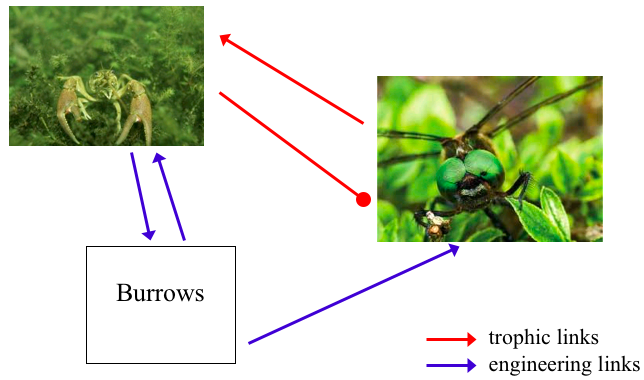
\includegraphics[width=0.5\linewidth]{hinescrayfish} \end{center}
\end{block}

\begin{block}{Models without mechanism cannot reliably extrapolate to
novel conditions}
\protect\hypertarget{models-without-mechanism-cannot-reliably-extrapolate-to-novel-conditions}{}
\end{block}

\begin{block}{Data-driven models usually lack mechanism}
\protect\hypertarget{data-driven-models-usually-lack-mechanism}{}
\begin{itemize}
\tightlist
\item
  statistical and machine-learning models can only make predictions that
  relate to patterns within the data supplied
\end{itemize}

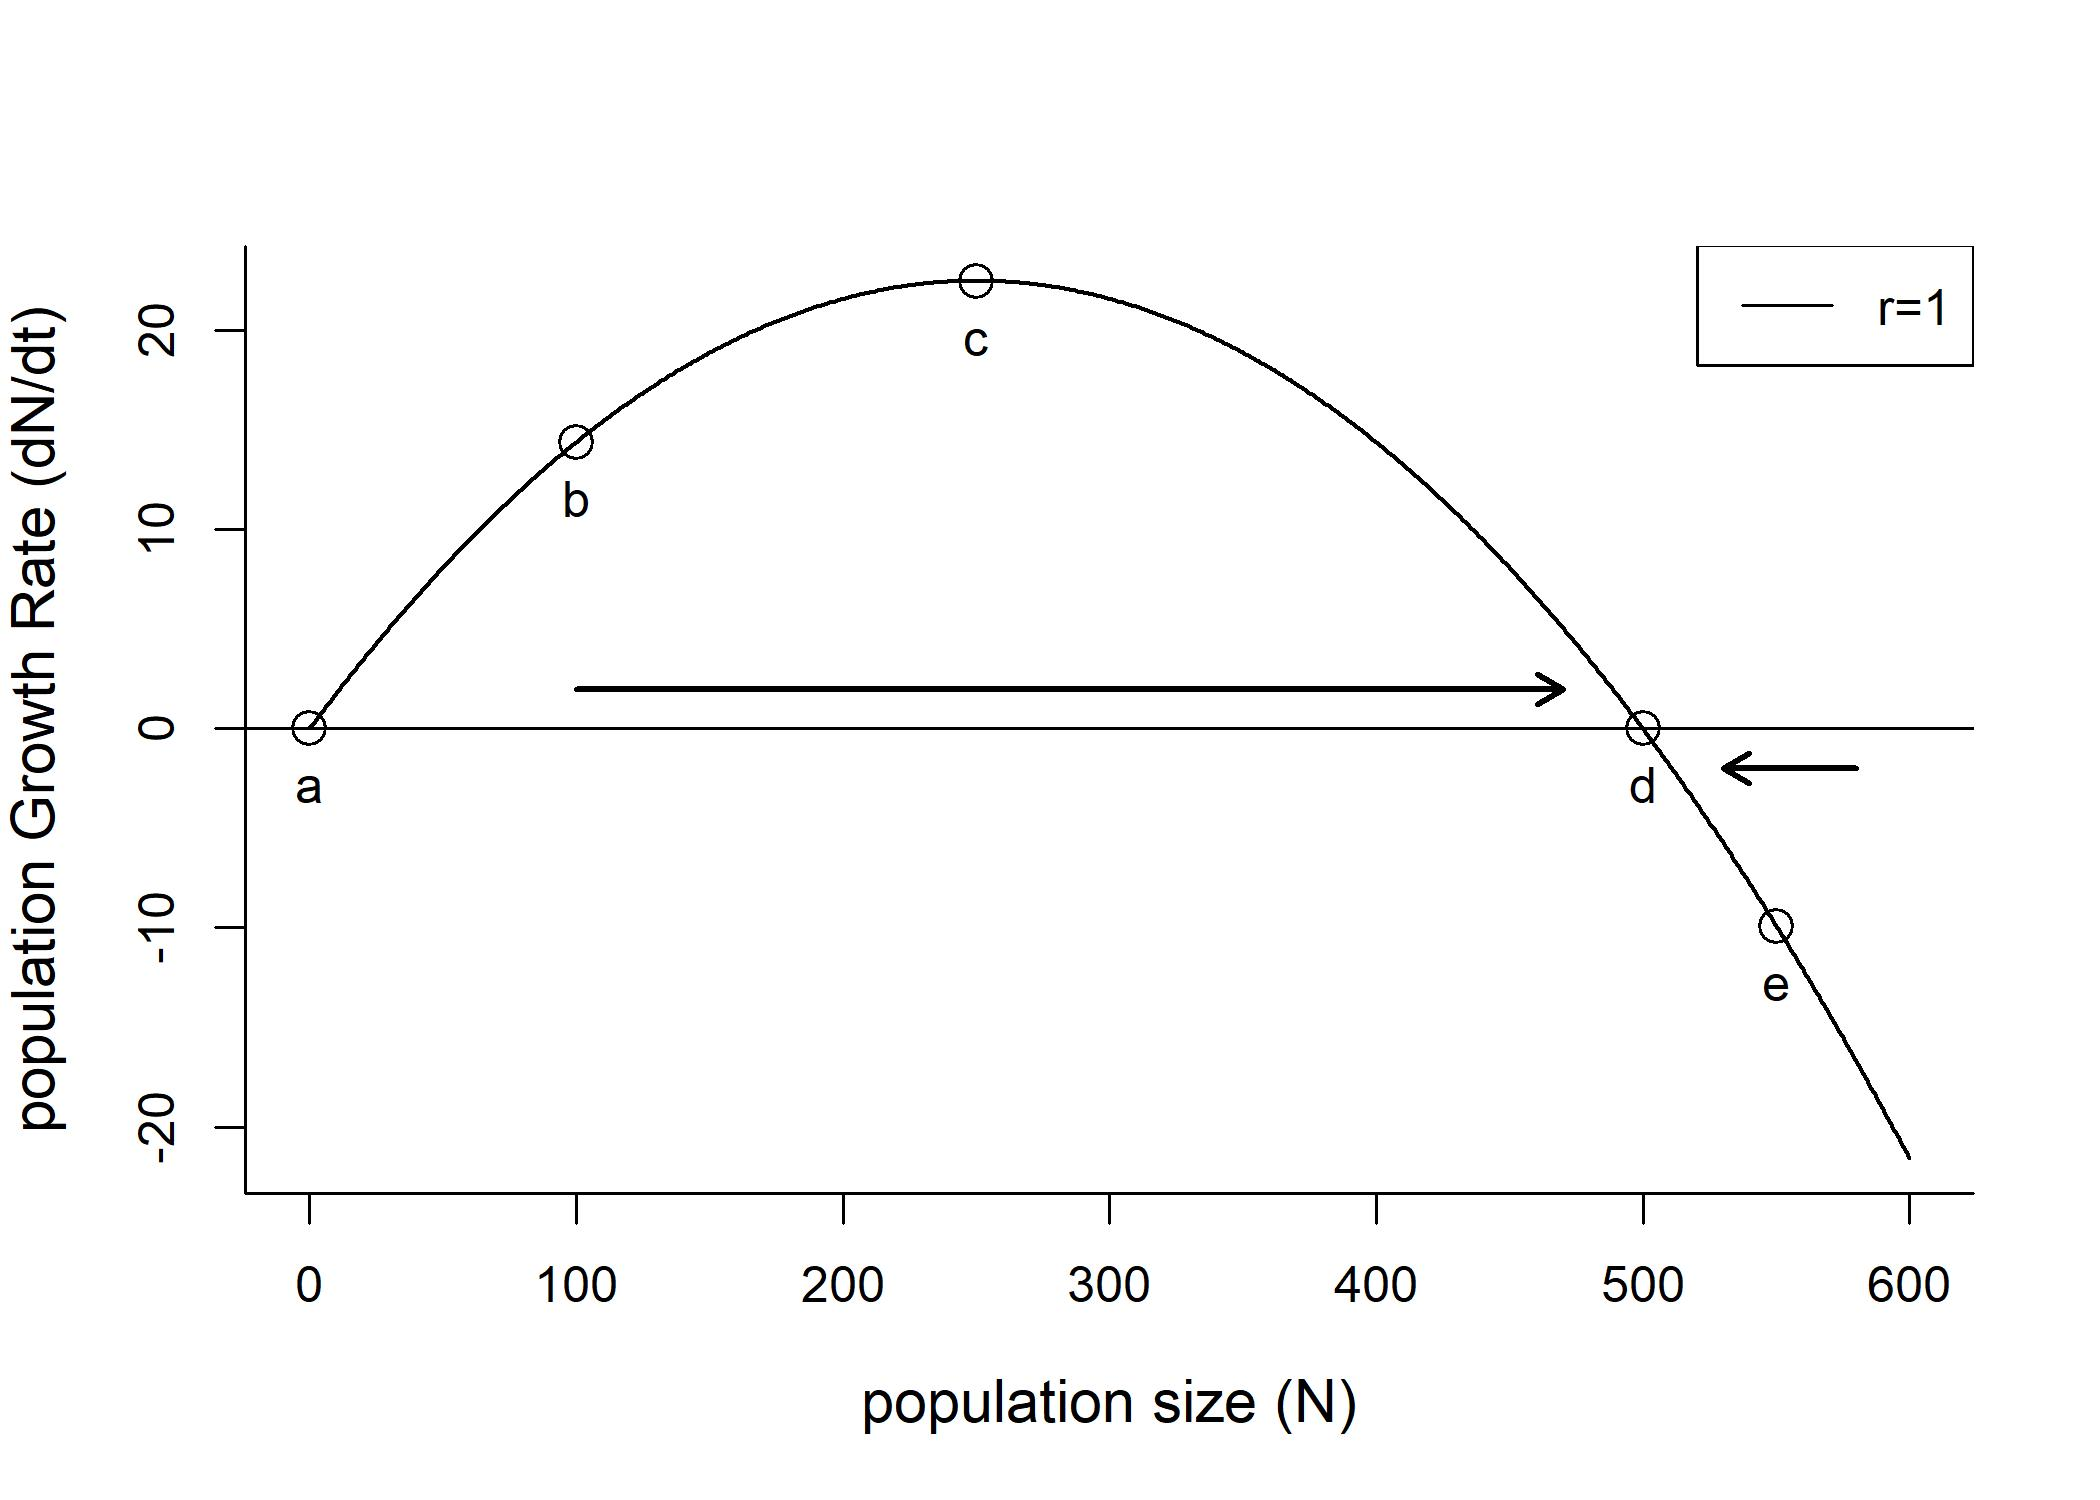
\includegraphics{datatheory_files/figure-beamer/unnamed-chunk-3-1.pdf}
\end{block}
\end{frame}

\begin{frame}{can we use data-driven models to develop mechanistic
explanations?}
\protect\hypertarget{can-we-use-data-driven-models-to-develop-mechanistic-explanations}{}
\begin{block}{Maxent algorithm}
\protect\hypertarget{maxent-algorithm}{}
\begin{itemize}
\tightlist
\item
  a machine learning method, which iteratively builds multiple models.
  It has two main components:
\end{itemize}

\begin{enumerate}
\item
  Entropy: the model is calibrated to find the distribution that is most
  spread out, or closest to uniform throughout the study region.
\item
  Constraints: the rules that constrain the predicted distribution.
  These rules are based on the values of the environmental variables
  (called features) of the locations where the species has been
  observed.
\end{enumerate}

\begin{flushright}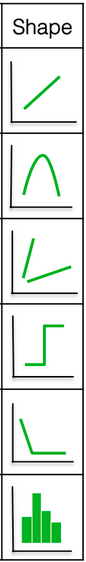
\includegraphics[width=0.4\linewidth]{Maxent} \end{flushright}
\end{block}

\begin{block}{Maxent modelling for giant hogweed distribution}
\protect\hypertarget{maxent-modelling-for-giant-hogweed-distribution}{}
\begin{itemize}
\item
  use experimental data to suggest candidate predictors: may require
  cold stratification, refer moist sites
\item
  intial Maxent model to find strong candidates and eliminate correlated
  predictors (normally we would leave these in and assume that the
  penalization would takec are of correlation)
\end{itemize}

\begin{center}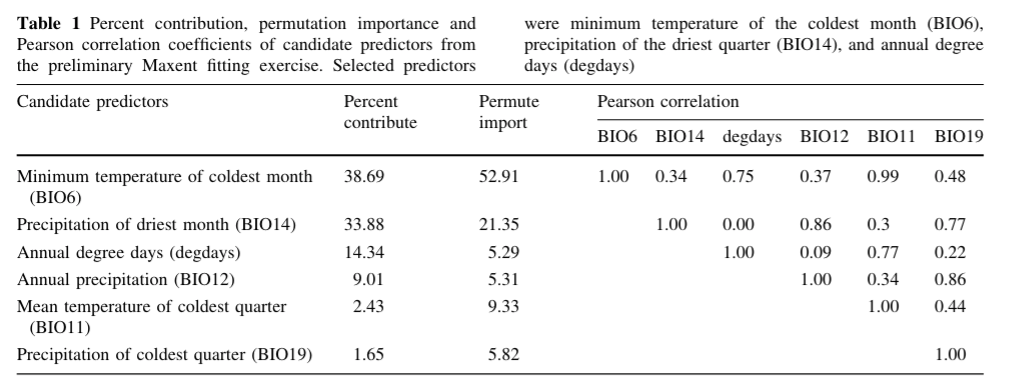
\includegraphics[width=1\linewidth]{tblehogweed} \end{center}
\end{block}

\begin{block}{Develop data-driven models, with an eye to mechanism}
\protect\hypertarget{develop-data-driven-models-with-an-eye-to-mechanism}{}
\begin{itemize}
\tightlist
\item
  constraint Maxent functions to forms that mimic standard ecothermic
  relationships (again, these are data-based)
\item
  train on a global dataset, test in inside and outside of training data
  range
\end{itemize}
\end{block}

\begin{block}{Data-driven models which suggest mechanism}
\protect\hypertarget{margins}{}
\begin{itemize}
\tightlist
\item
  final set of simple maxent models, and related statistical
  model\ldots.
\end{itemize}

\begin{center}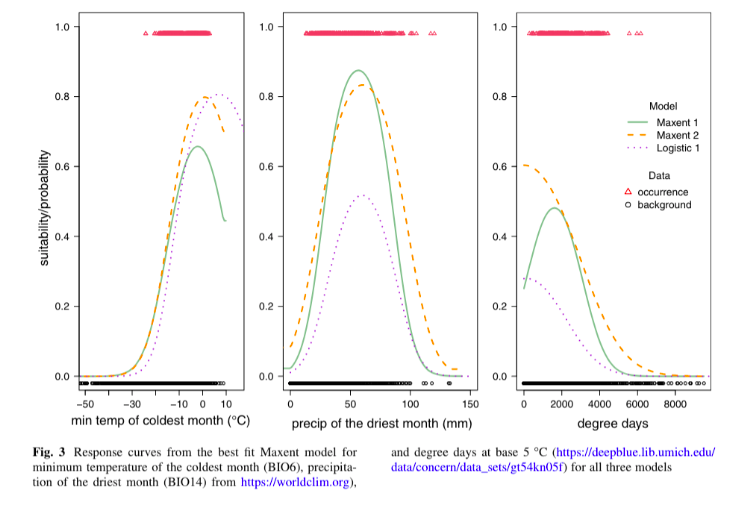
\includegraphics[width=0.8\linewidth]{modelshogweed} \end{center}

\href{https://doi.org/10.1007/s10530-021-02645-x}{Cuddington et
al.~(2022)}

`
\end{block}

\begin{block}{Let's use data-driven modelling to identify mechanism}
\protect\hypertarget{lets-use-data-driven-modelling-to-identify-mechanism}{}
\begin{itemize}
\tightlist
\item
  giant hogweed: the beginnings of a mechanistic model:

  \begin{itemize}
  \tightlist
  \item
    requirements for cold seed stratification temperatures to break
    dormancy
  \item
    with development delays above this range
  \end{itemize}
\item
  does require constraints, previous experiment, and some logical
  connections
\end{itemize}
\end{block}
\end{frame}

\begin{frame}{can we use mechanistic models to better understand data?}
\protect\hypertarget{can-we-use-mechanistic-models-to-better-understand-data}{}
\begin{block}{Regime shifts in bistable systems}
\protect\hypertarget{margins2}{}
\begin{itemize}
\tightlist
\item
  a ``sudden'' change in state, e.g., Scheffer (2001)
  \(\frac{dx}{dt}=\frac{hx^\rho}{x^\rho+c}-b x+a\)
\item
  lake system moves from phytoplankton-dominated, eutrophic green water
  state to macrophyte-dominated, oligotrophic state
\end{itemize}

\begin{center}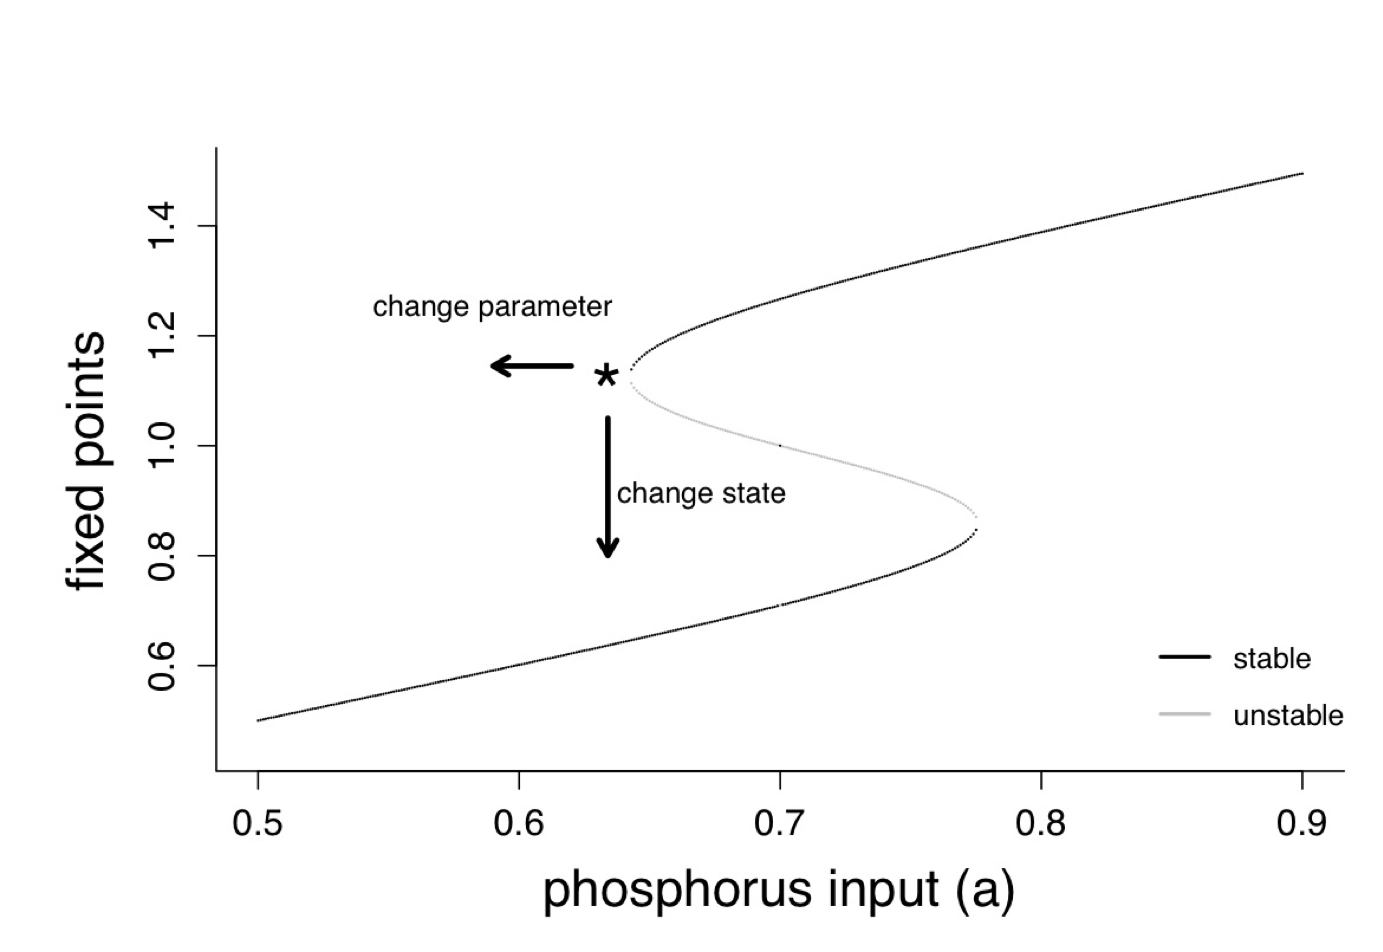
\includegraphics[width=0.7\linewidth]{schefferbifur} \end{center}

\href{https://www.nature.com/articles/s41559-020-01365-0}{Francis et
al.~(2021)}

`
\end{block}

\begin{block}{Two ways to get a regime shift}
\protect\hypertarget{two-ways-to-get-a-regime-shift}{}
\begin{enumerate}
\tightlist
\item
  Erode stability of one eq'm, or
\item
  Push system to second stable basin with a disturbance
\end{enumerate}

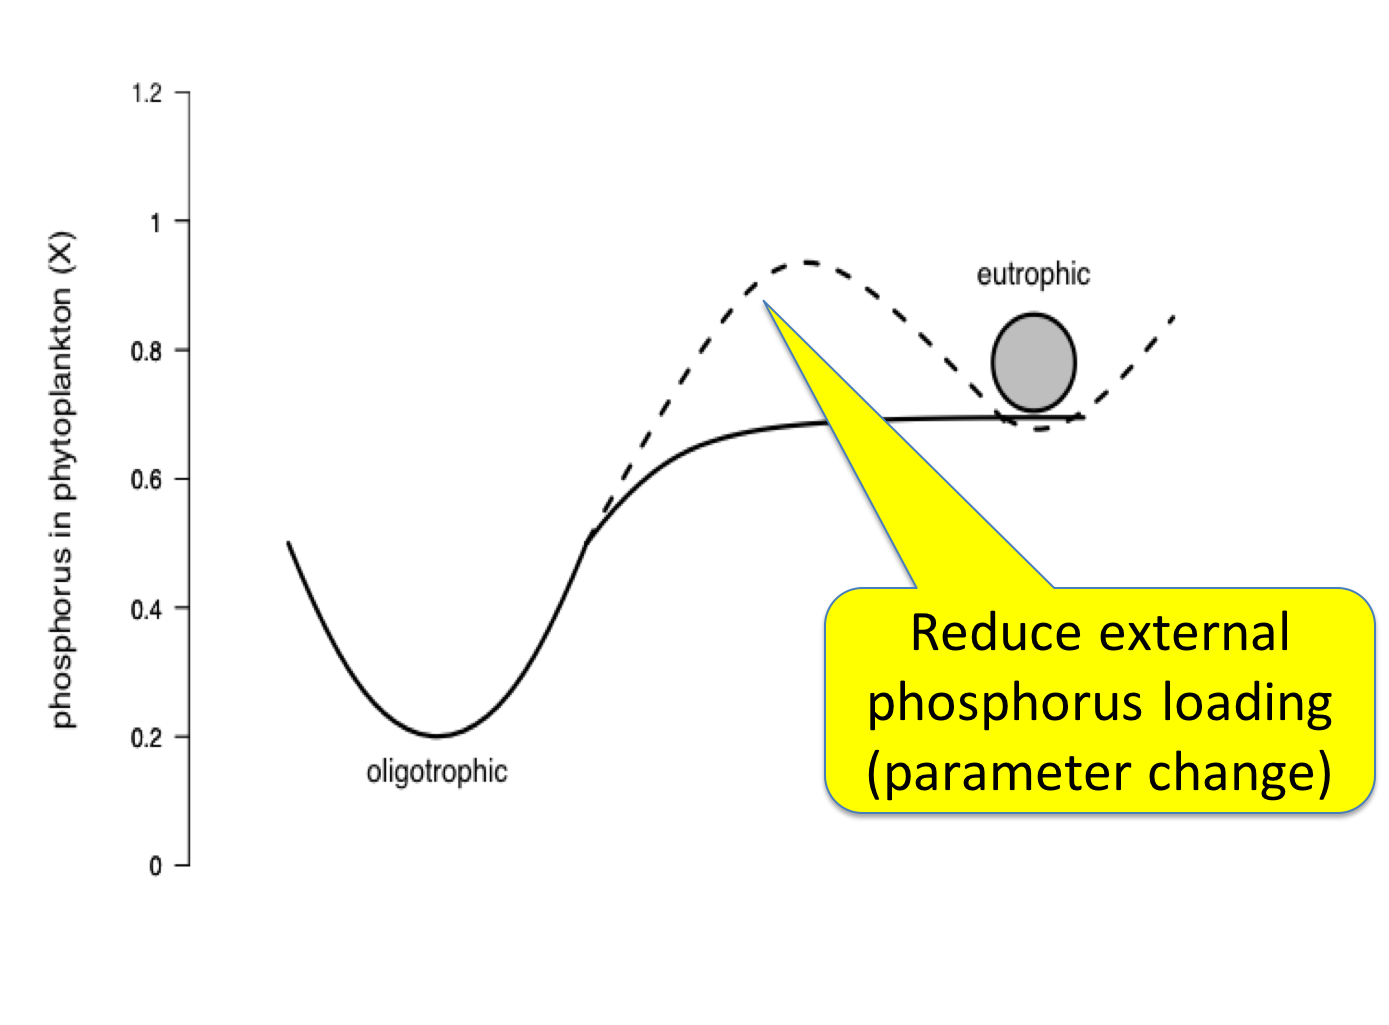
\includegraphics[width=0.5\linewidth]{schefferschematic}
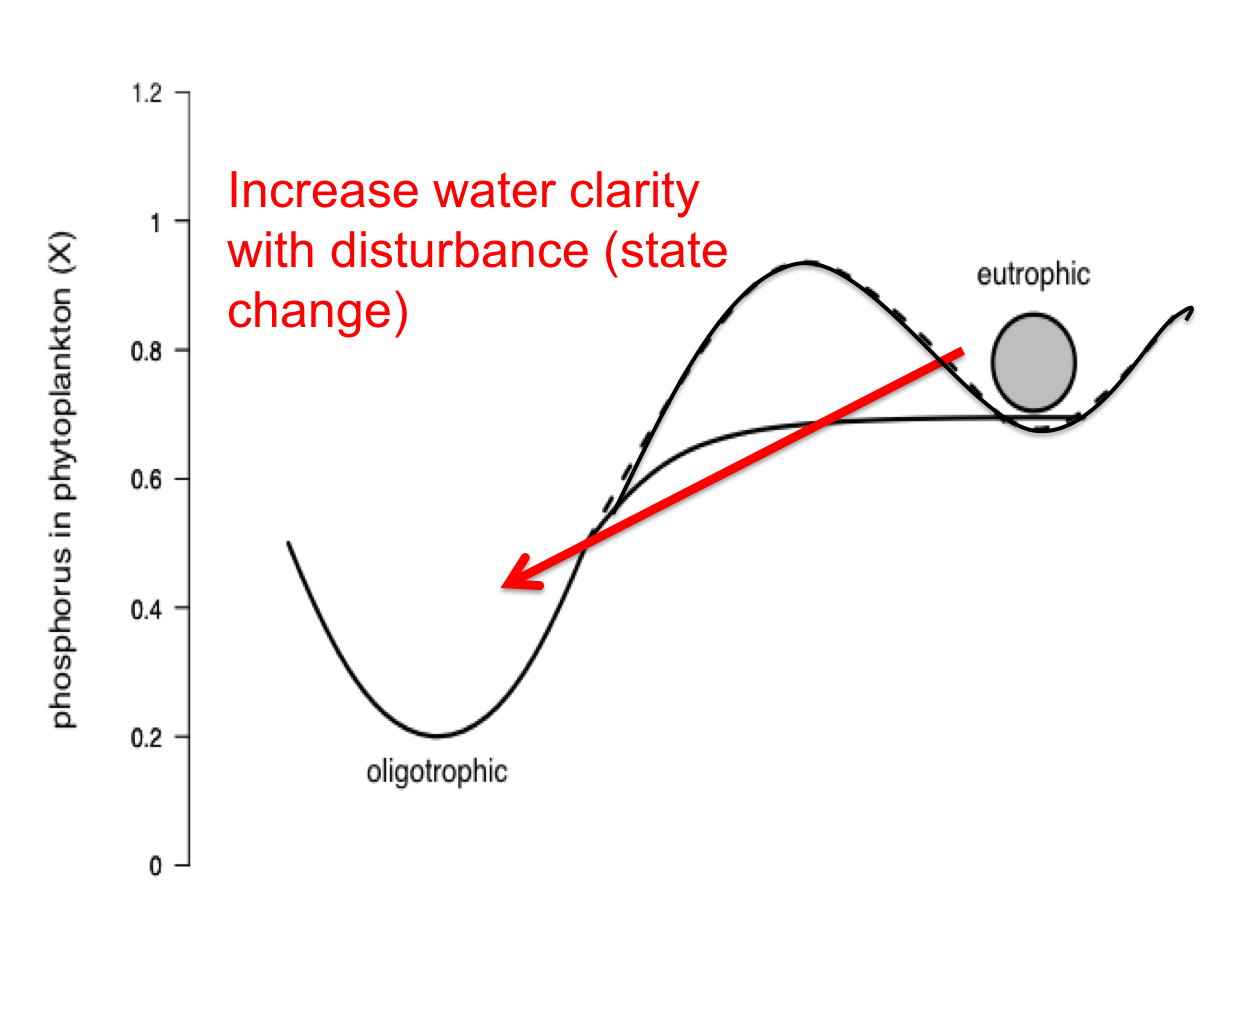
\includegraphics[width=0.5\linewidth]{schefferdisturb} \#\# Wait\ldots{}
is that all the mechanistic model predicts? -asymptotic vs transient
dynamics predicted by models

\begin{center}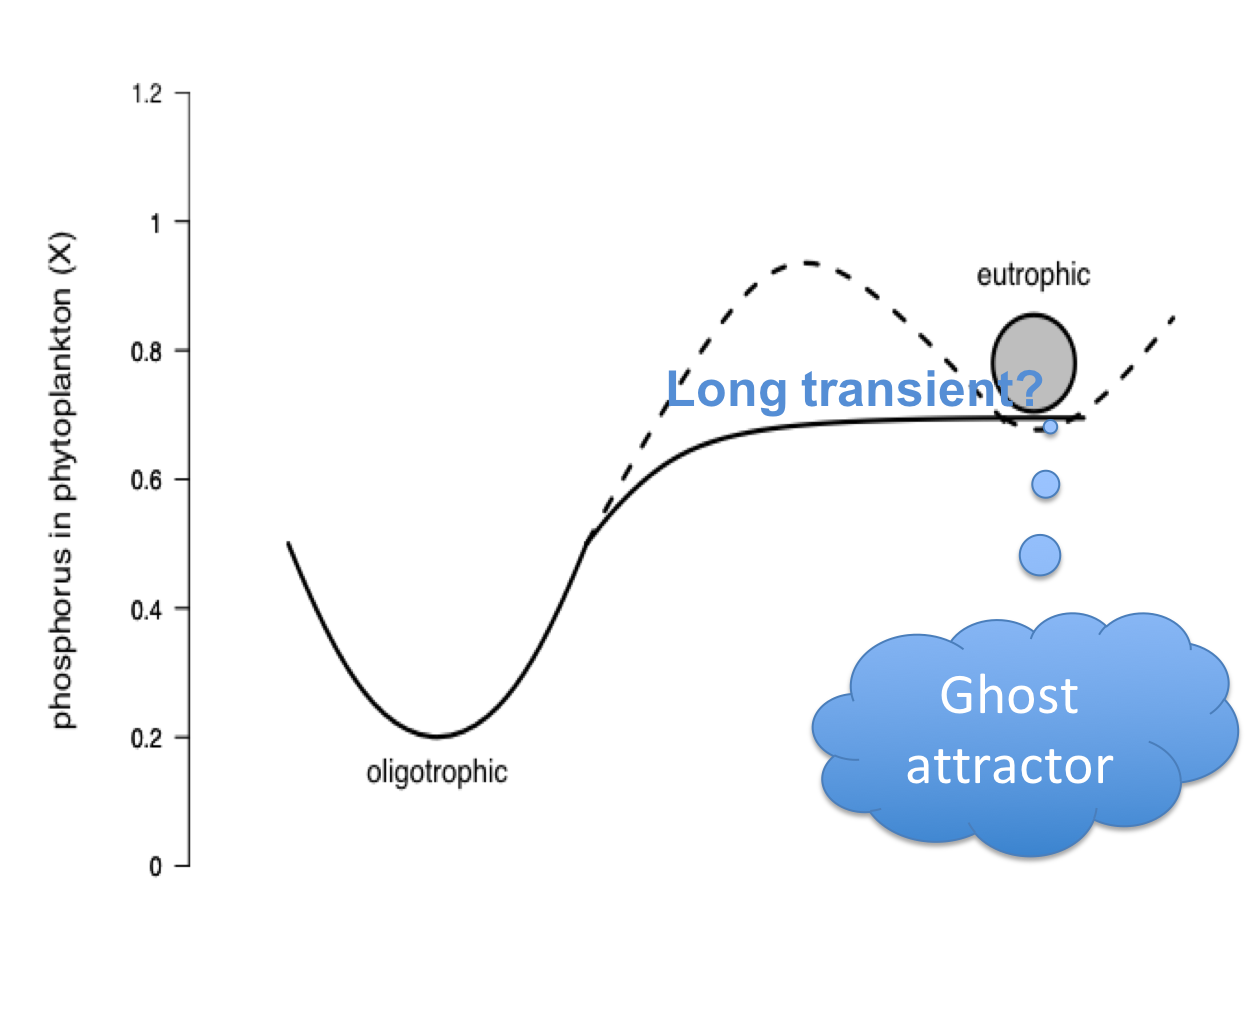
\includegraphics[width=0.7\linewidth]{schefferghost} \end{center}
\end{block}

\begin{block}{Bay of Quinte}
\protect\hypertarget{bay-of-quinte}{}
\begin{itemize}
\tightlist
\item
  history of being increasingly eutrophic
\item
  phosophorus controls inplemented 1978
\item
  invaded by zebra mussels in 1994
\item
  meostrophic following this
\end{itemize}

\begin{figure}
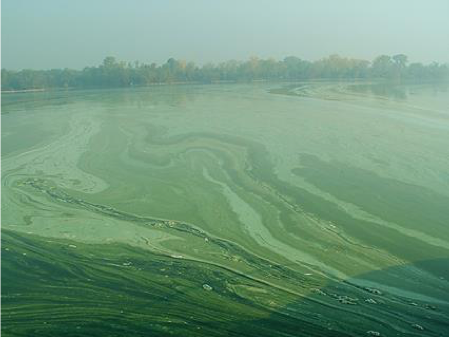
\includegraphics[width=0.4\linewidth]{turbid} 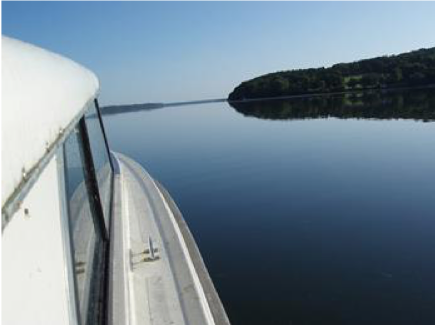
\includegraphics[width=0.4\linewidth]{clear} \caption{Bay of Quinte before and after mussel invasion}\label{fig:unnamed-chunk-10}
\end{figure}
\end{block}

\begin{block}{Standard explanation: Disturbance shift to new stable
state}
\protect\hypertarget{standard-explanation-disturbance-shift-to-new-stable-state}{}
``In the mid-1990s, zebra and quagga mussels (Dreissena spp.) invaded
the area, \textbf{dramatically changing the water clarity because of the
filter-feeding capacity.}''

Bay of Quinte remedial action plant (2017)
\end{block}

\begin{block}{Long transients in a regime shift model}
\protect\hypertarget{long-transients-in-a-regime-shift-model}{}
-long transients can be a quite common prediction

\begin{center}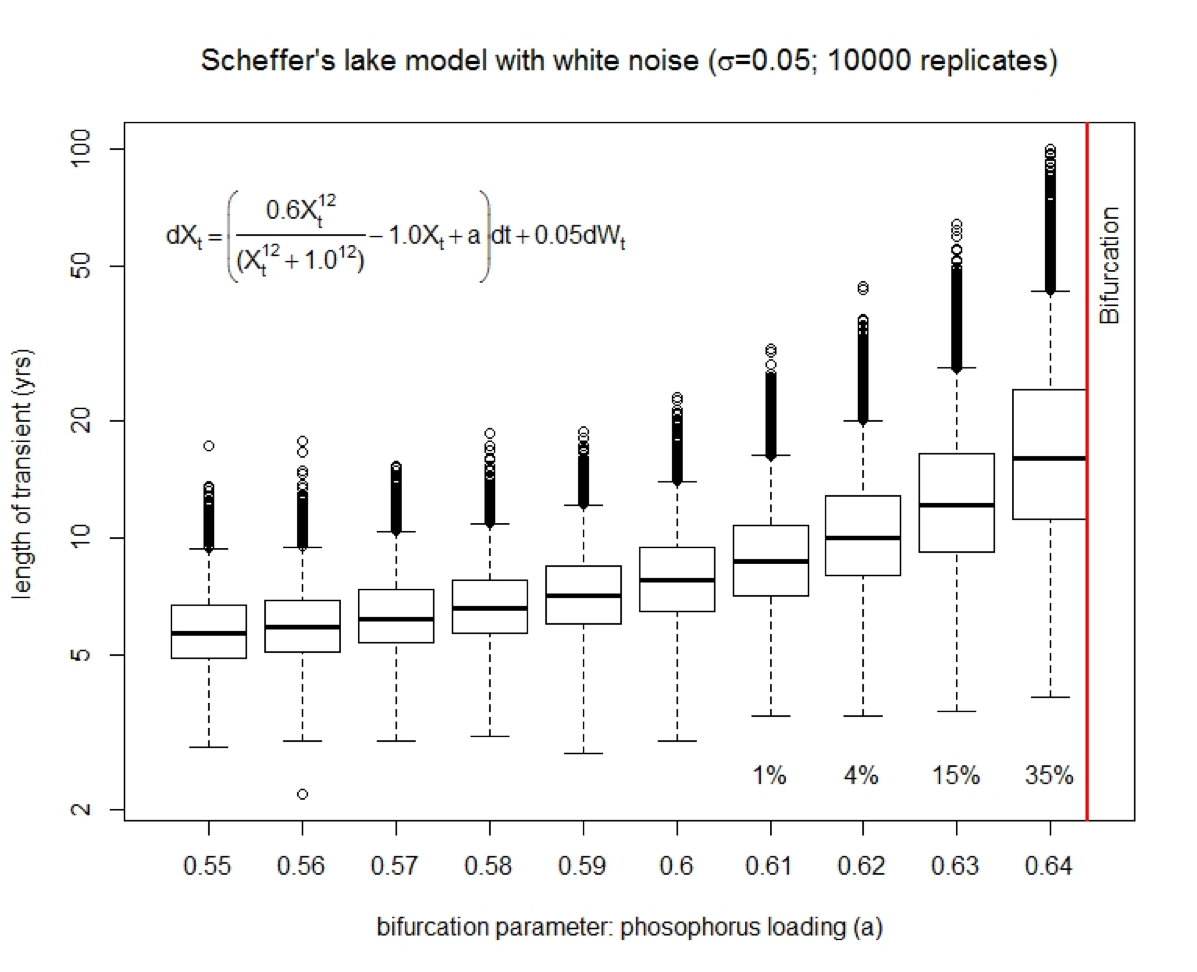
\includegraphics[width=0.7\linewidth]{transbox} \end{center}

\href{}{Currie \& Cuddington, in prep}

`
\end{block}

\begin{block}{Alternative explanations for change in Bay of Quinte}
\protect\hypertarget{alternative-explanations-for-change-in-bay-of-quinte}{}
\begin{itemize}
\item
  all of which arise from the SAME mechanistic model

  \begin{enumerate}
  \tightlist
  \item
    a regime shift to a 2nd stable state cause by the disturbance of the
    zebra mussel invasions
  \item
    a long transient following the erosion of the the stability of the
    eutrophic state because of a lingering ghost attractor
  \item
    there was just a slow change in phosphorus (i.e.~the system does not
    have bistable dynamics)
  \end{enumerate}
\end{itemize}
\end{block}

\begin{block}{Examine alternatives using data-driven models:}
\protect\hypertarget{examine-alternatives-using-data-driven-models}{}
\begin{itemize}
\tightlist
\item
  Linear breakpoint analysis \(E(y_i)=β_0+break_i+x_i\)
\item
  Nonlinear analysis: Use generalized additive model (GAM:
  \(E(y_i)=β_0+f(x_i)\)), and examine the first derivative of fitted
  smooth to find periods of rapid change
\end{itemize}

Simulated data from Scheffer model (2001) where the high turbidity
state, which is the initial condition, is no longer stable, showing the
timeseries (points), fitted GAM model (black line) and 95\% credible
interval (green lines) for three different levels of additive noise
(a-c), then taking the first derivative (d-f) of fitted GAM (black
line), with simultaneous confidence intervals (green lines). Where the
derivative significantly deviates from zero, we have a period of rapid
change.

\begin{center}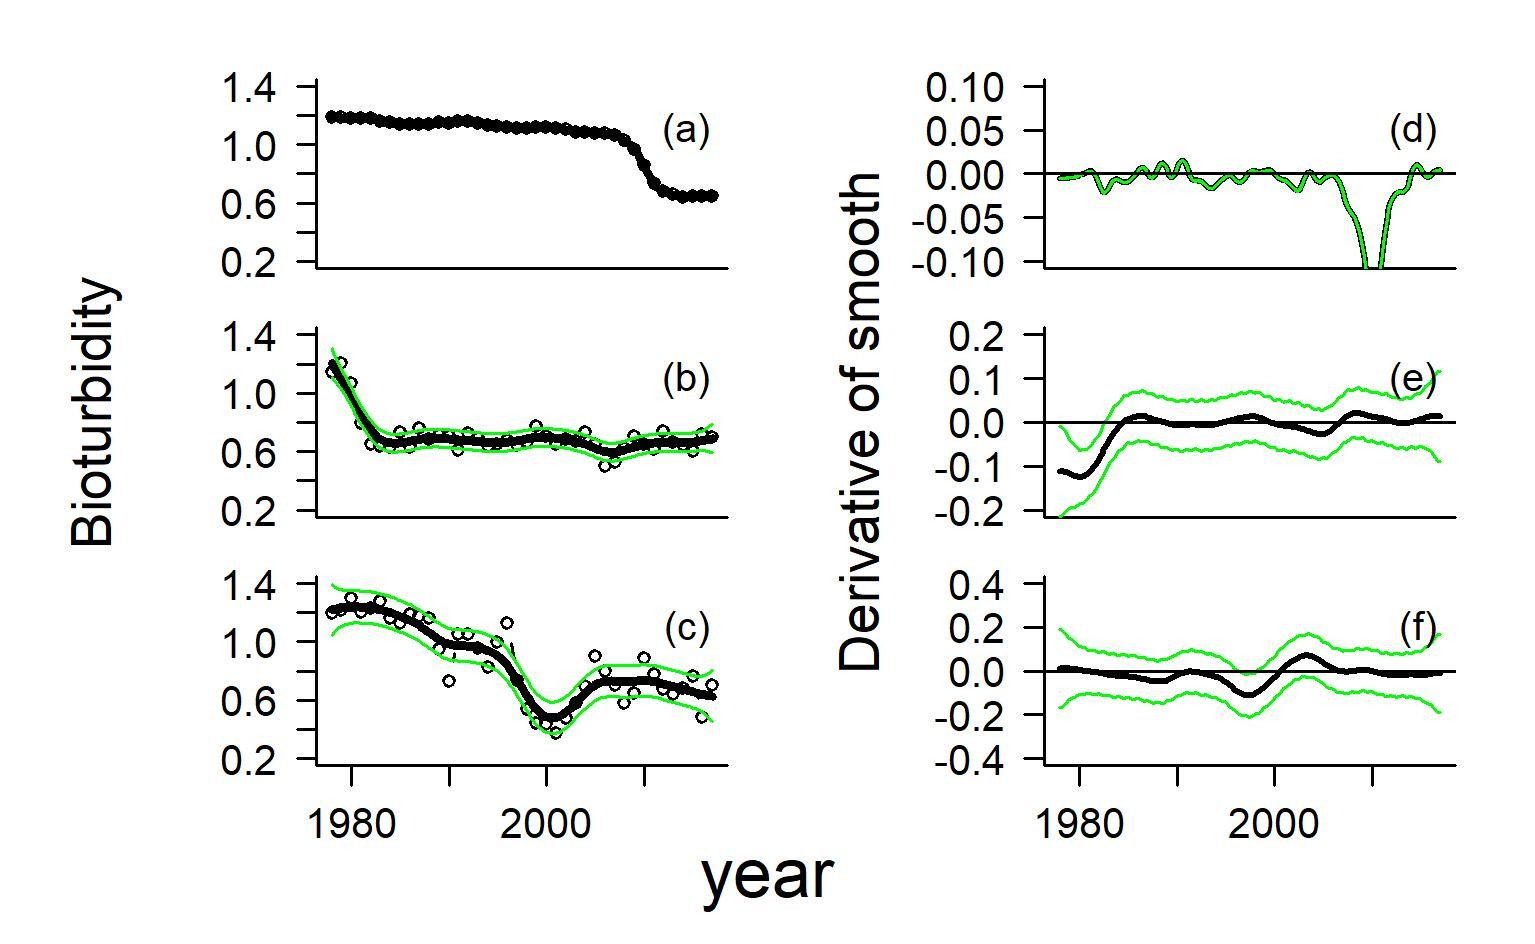
\includegraphics[width=0.9\linewidth]{schaefferexap} \end{center}

\href{}{Currie \& Cuddington, in prep}

`
\end{block}

\begin{block}{1. examine the dynamics of a mechanistic driver
(phosphorus)}
\protect\hypertarget{examine-the-dynamics-of-a-mechanistic-driver-phosphorus}{}
\begin{itemize}
\tightlist
\item
  rapid response to management in the 70s
\item
  slow change after that
\end{itemize}

\begin{center}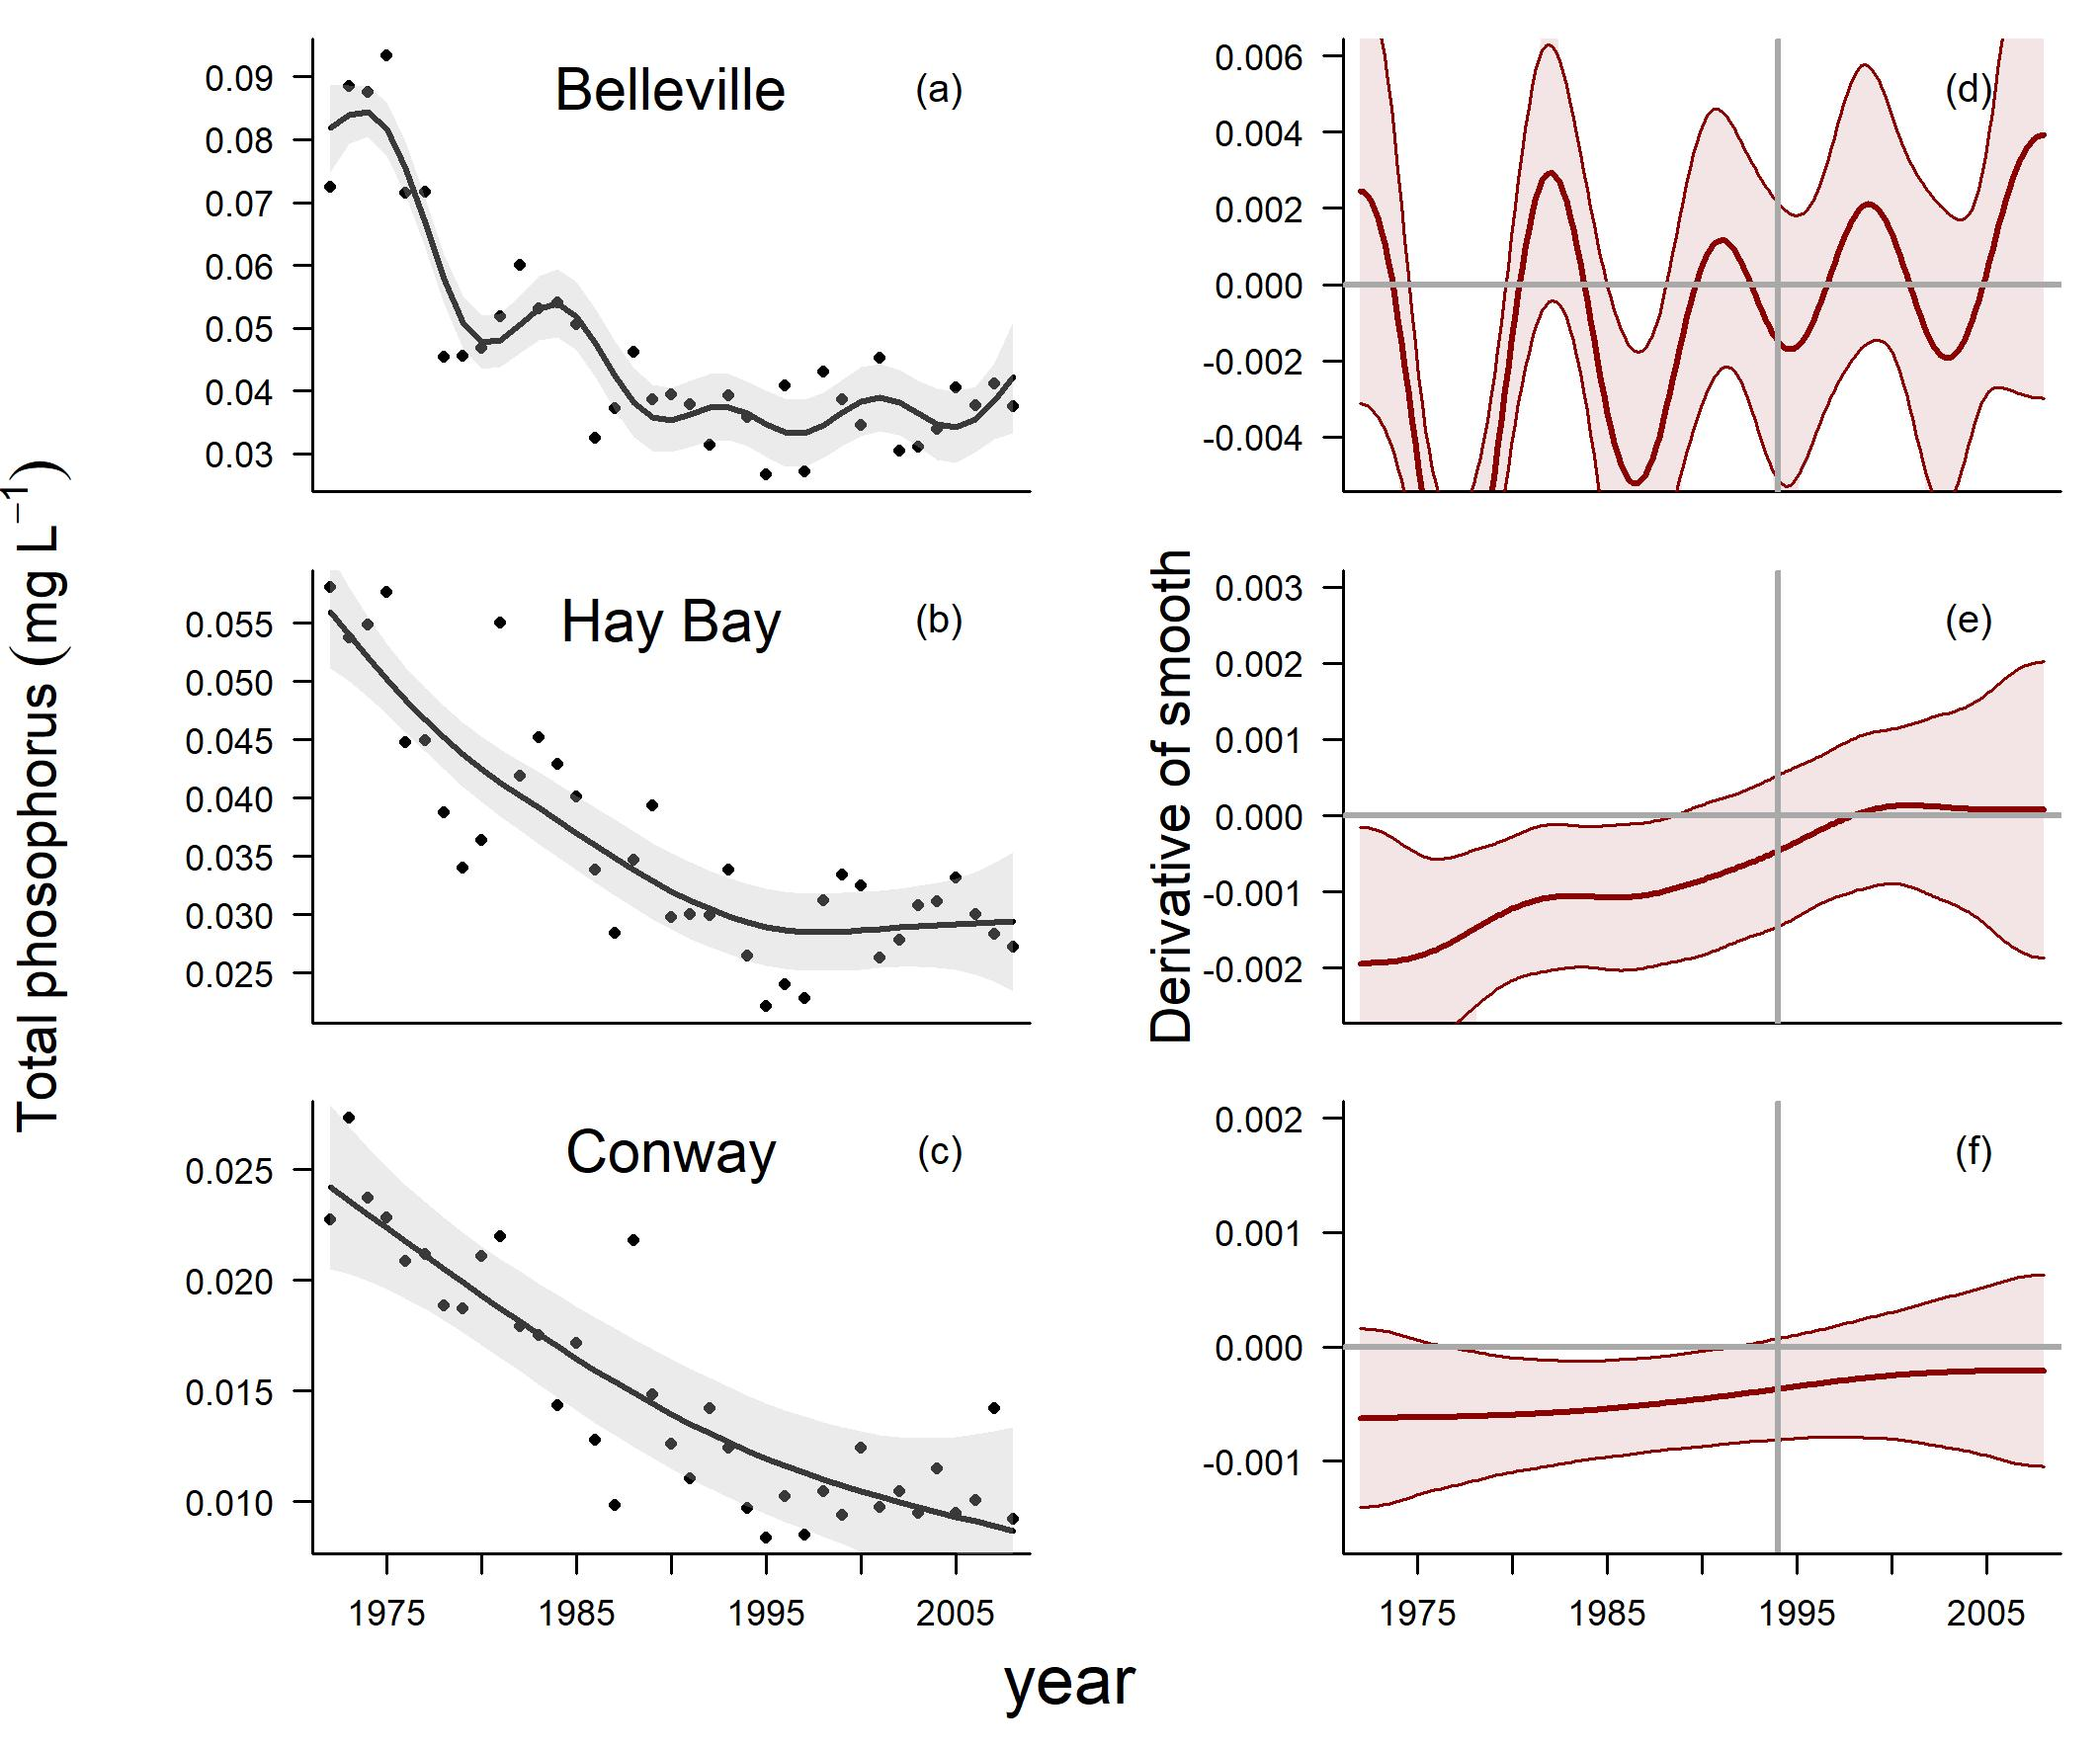
\includegraphics[width=1\linewidth]{TPgamApr08} \end{center}

\begin{center}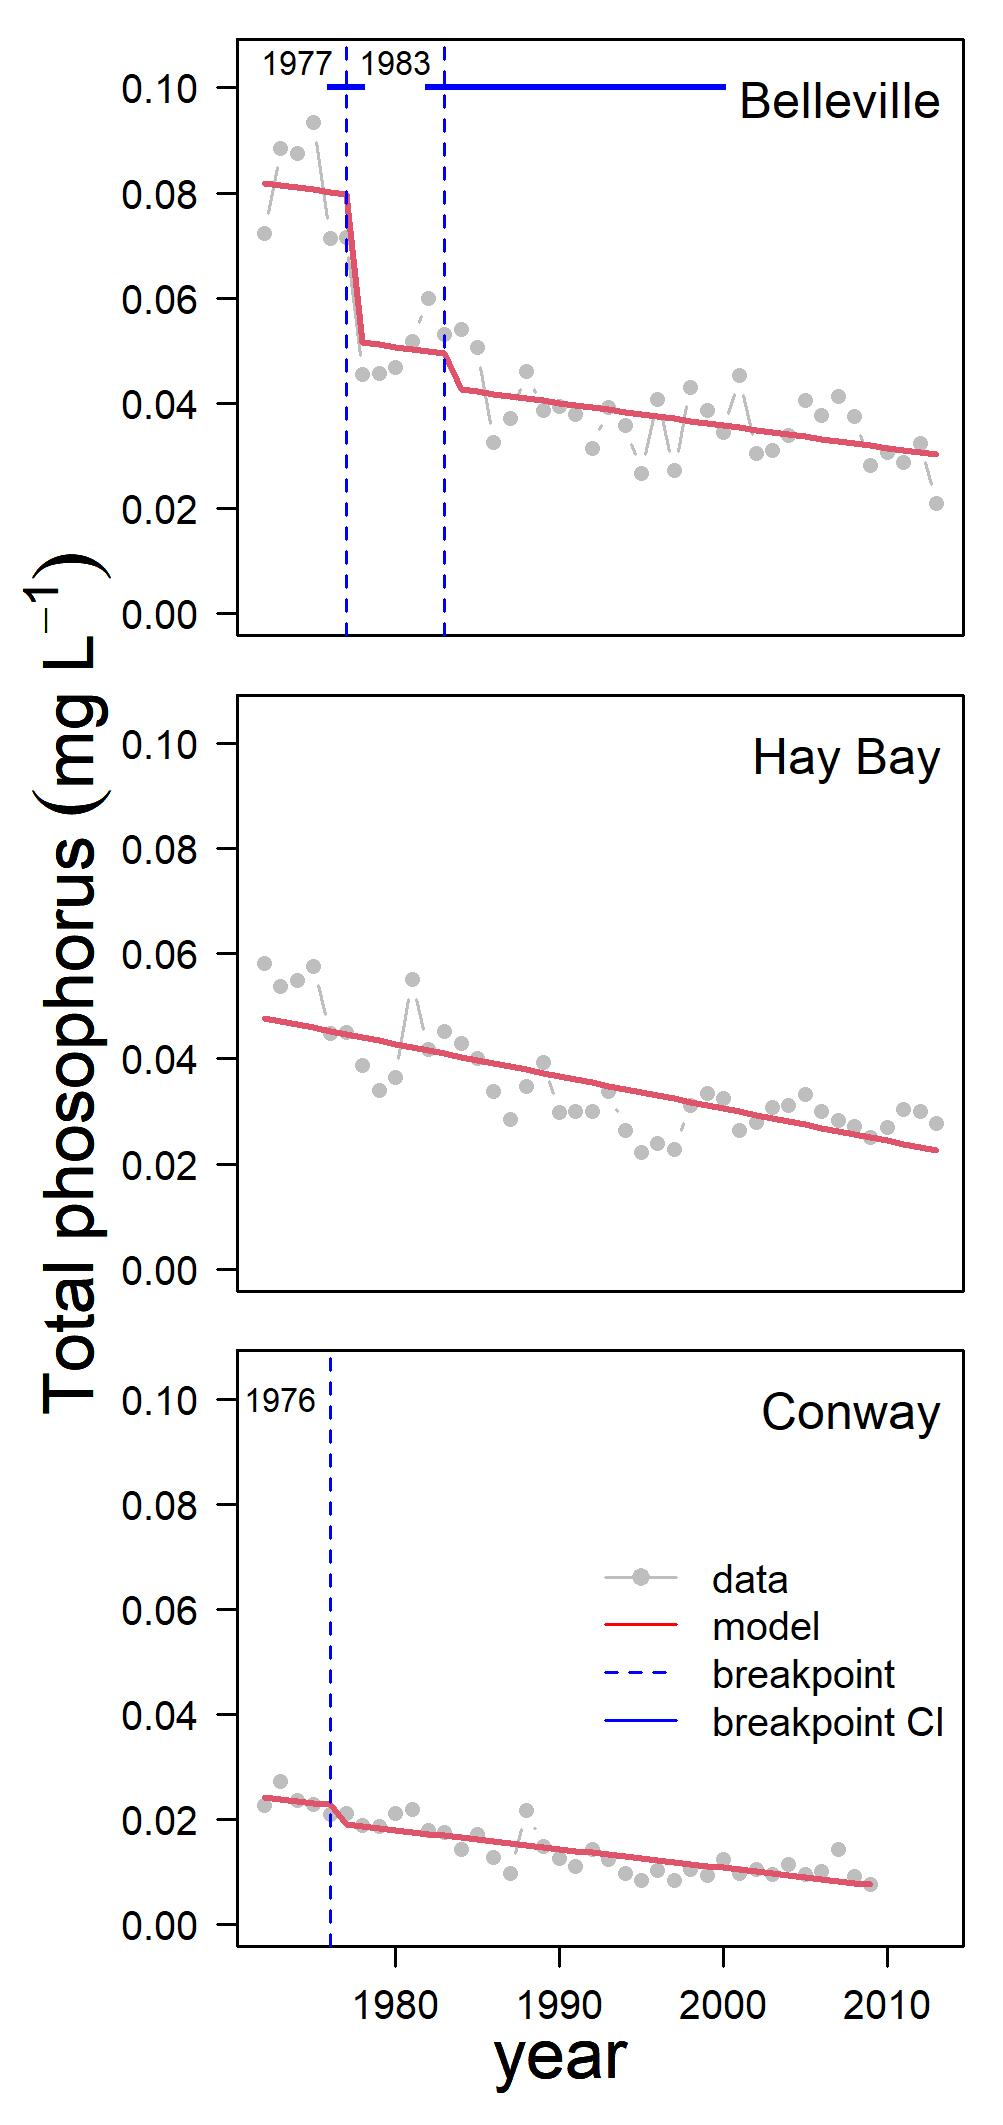
\includegraphics[width=0.6\linewidth]{TPbreak} \end{center}

\href{}{Currie \& Cuddington, in prep}

`
\end{block}

\begin{block}{2. examine the dynamics of the disturbance (zebra
mussels)}
\protect\hypertarget{examine-the-dynamics-of-the-disturbance-zebra-mussels}{}
\begin{itemize}
\tightlist
\item
  mussel veligers first detected in 1994
\item
  very low densities
\end{itemize}

\begin{center}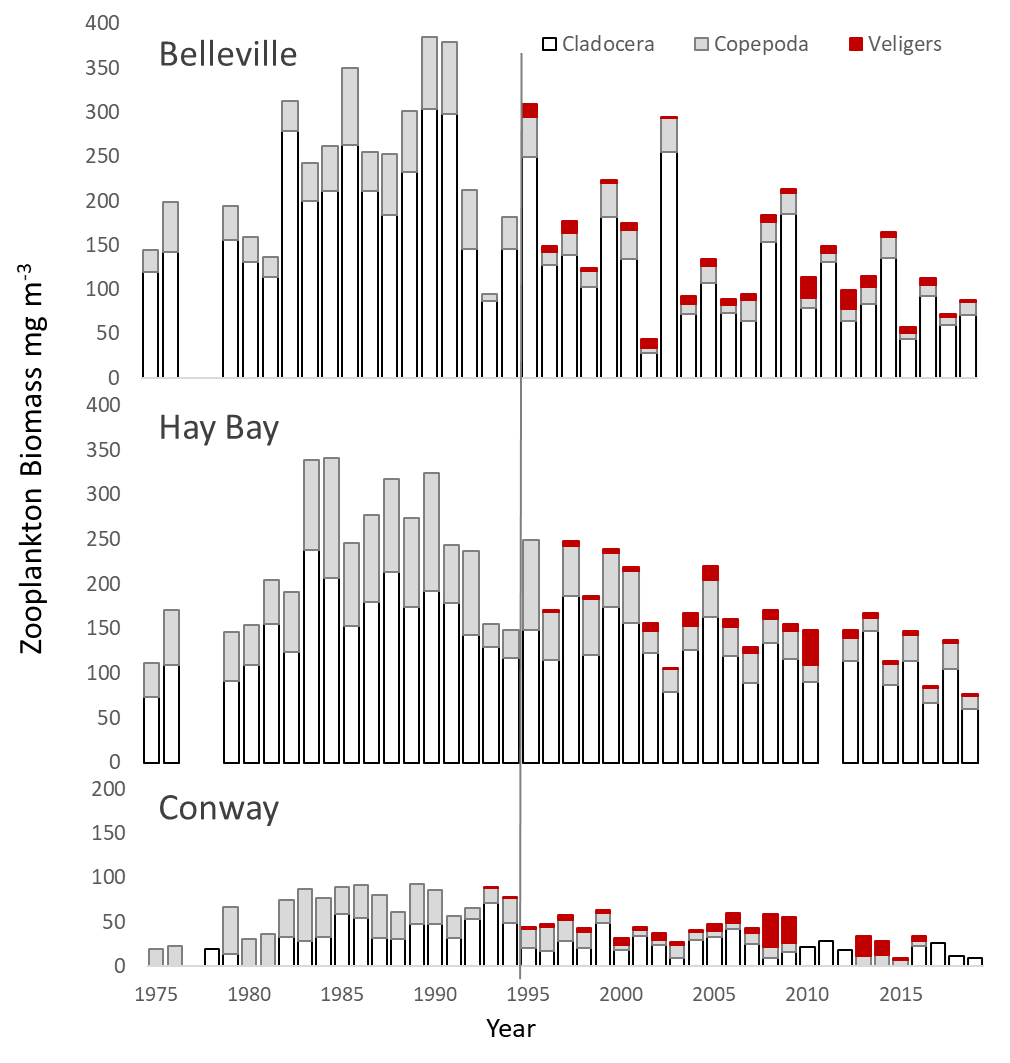
\includegraphics[width=0.8\linewidth]{zoobar} \end{center}

\href{}{Currie \& Cuddington, in prep}

`
\end{block}

\begin{block}{3. examine the dynamics of the response (water clarity)}
\protect\hypertarget{margins}{}
\begin{itemize}
\tightlist
\item
  linear breakpoint model
  \(E(light_{i,s}) = \beta_s+break period_{i,s} + year_{i,s} + TP_i\)
\item
  response to phosphorus controls in the 70s at Belleville
\item
  maybe rapid change after mussels at Hay Bay?
\end{itemize}

\begin{center}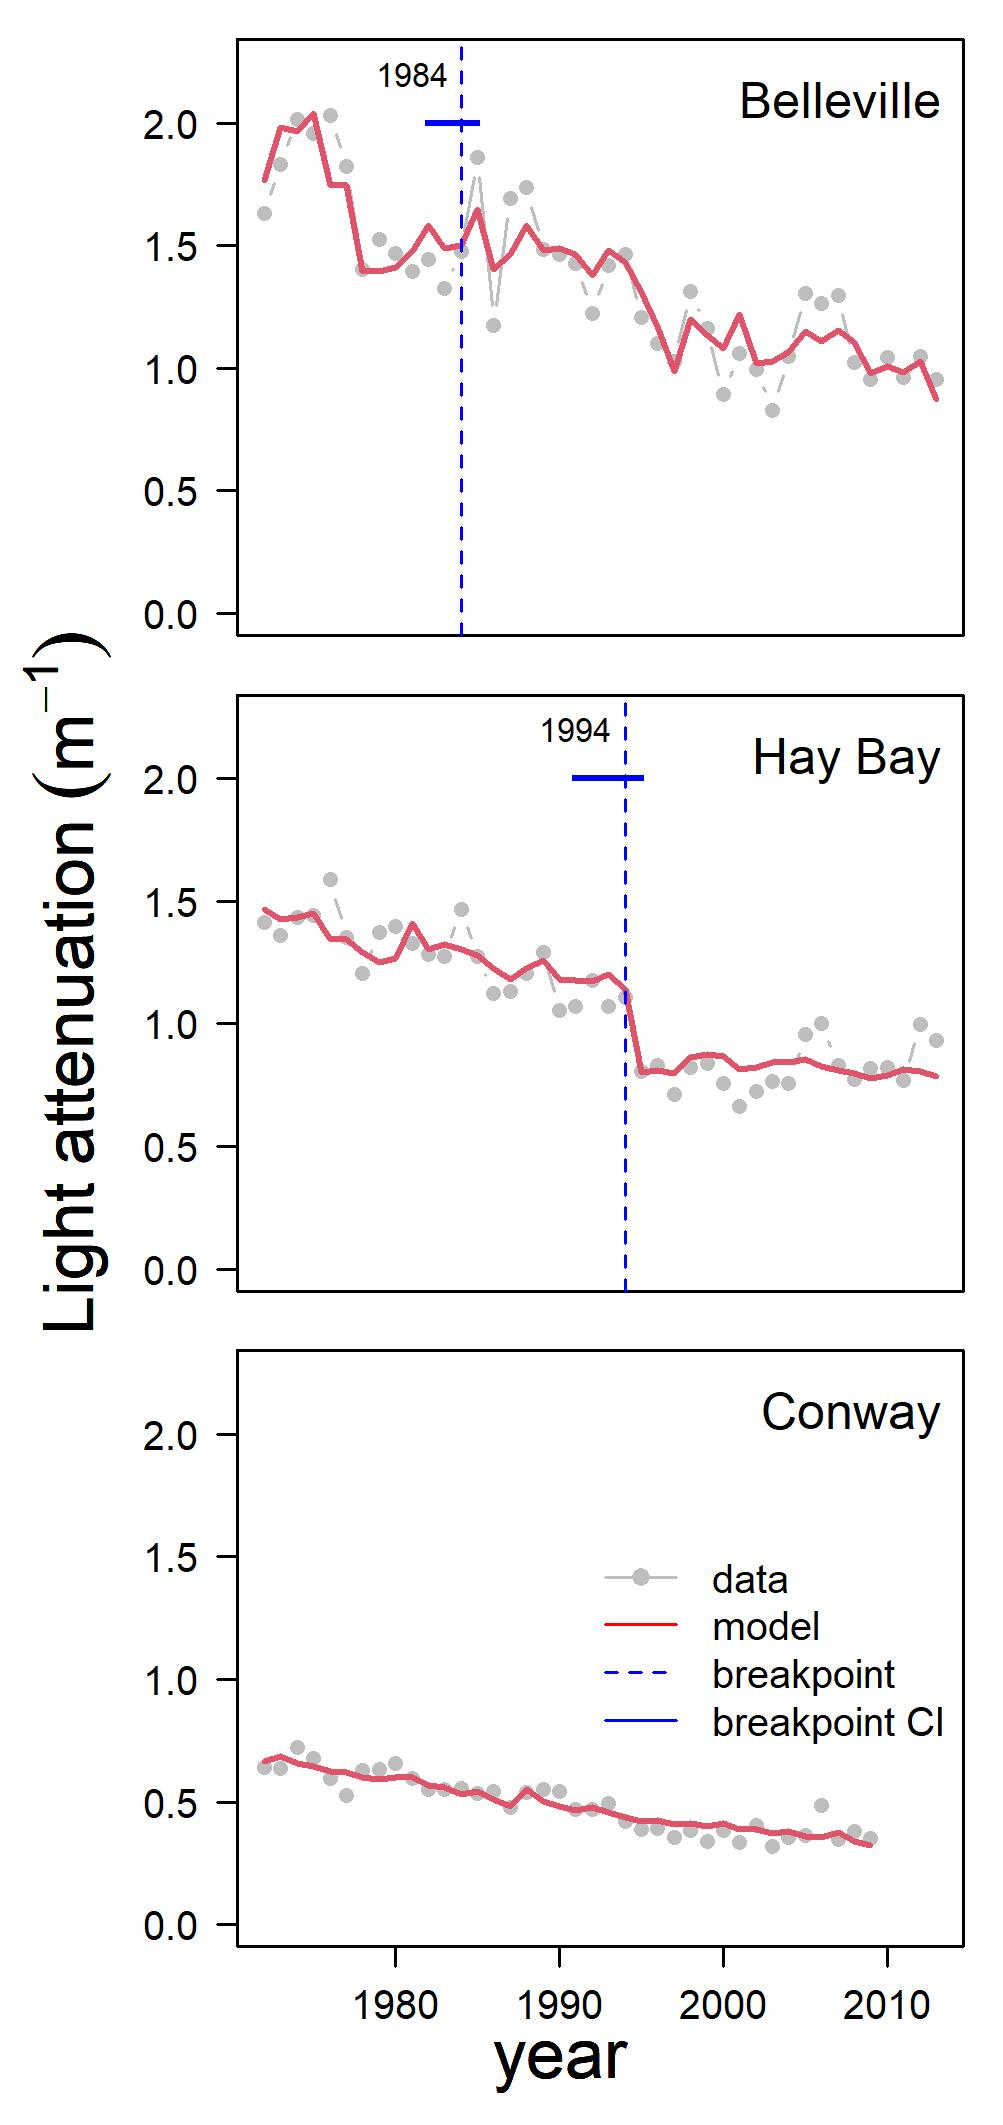
\includegraphics[width=0.5\linewidth]{lightbreakwgt} \end{center}

\href{}{Currie \& Cuddington, in prep}

`
\end{block}

\begin{block}{3. examine the dynamics of the response (water clarity)}
\protect\hypertarget{examine-the-dynamics-of-the-response-water-clarity}{}
\begin{itemize}
\tightlist
\item
  nonlinear analysis : \(E(light_{i,s})=β_s+f(year_{i,s})+f(TP_i)\)
\item
  suggests rapid change at Belleville and Hay Bay
\item
  rapid change magnitude becomes pretty small when we control for
  concurvity in phosphorus impacts
\end{itemize}

\begin{center}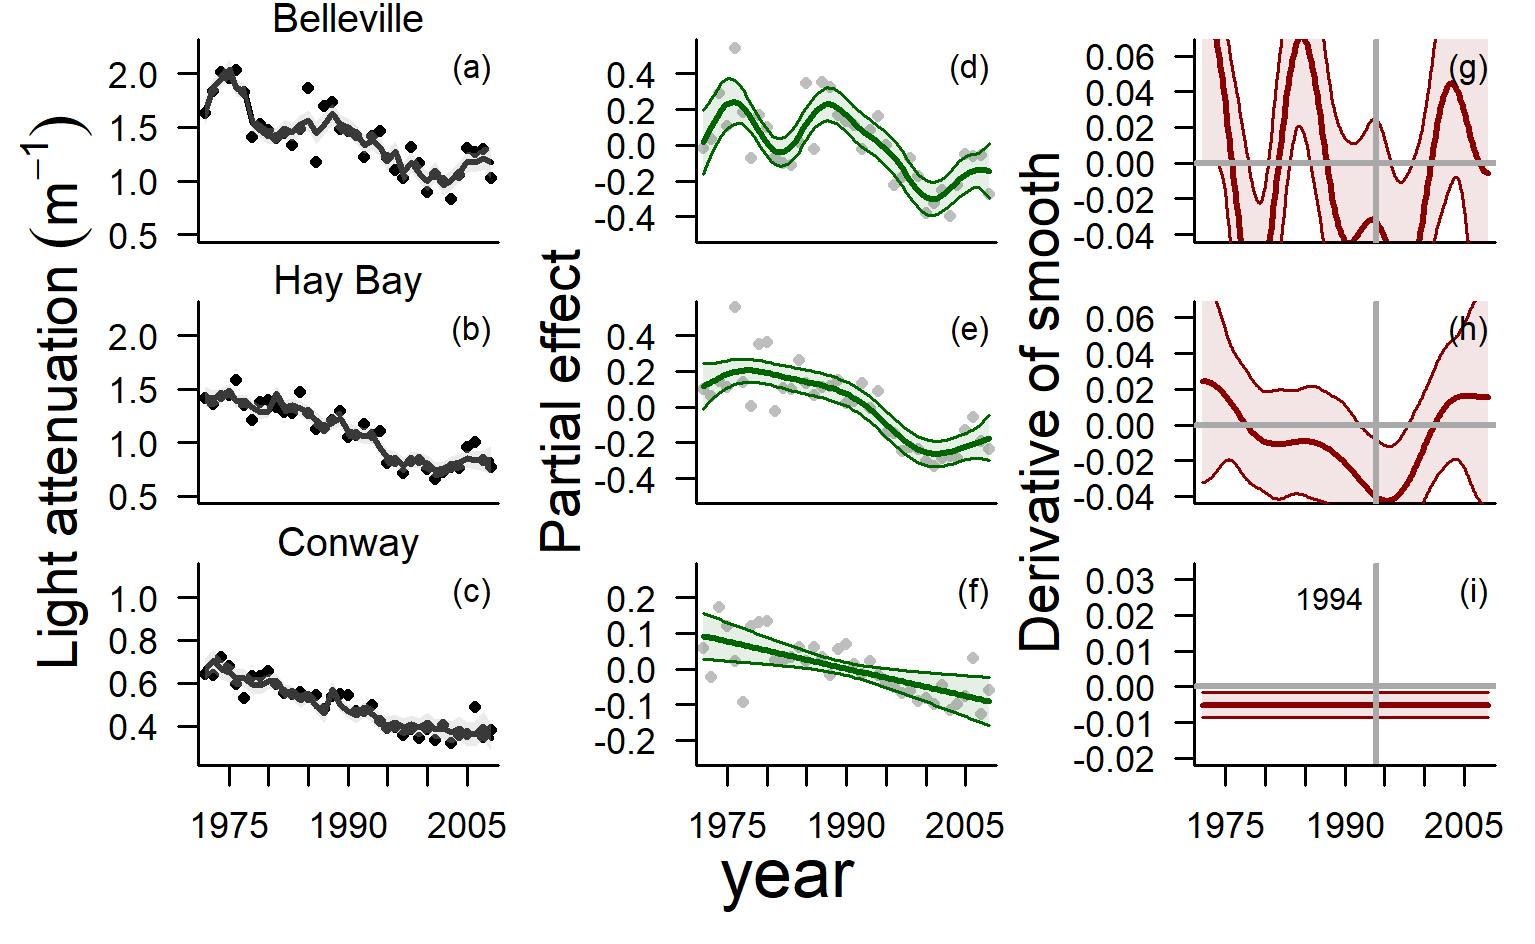
\includegraphics[width=0.7\linewidth]{lightgamApr11} 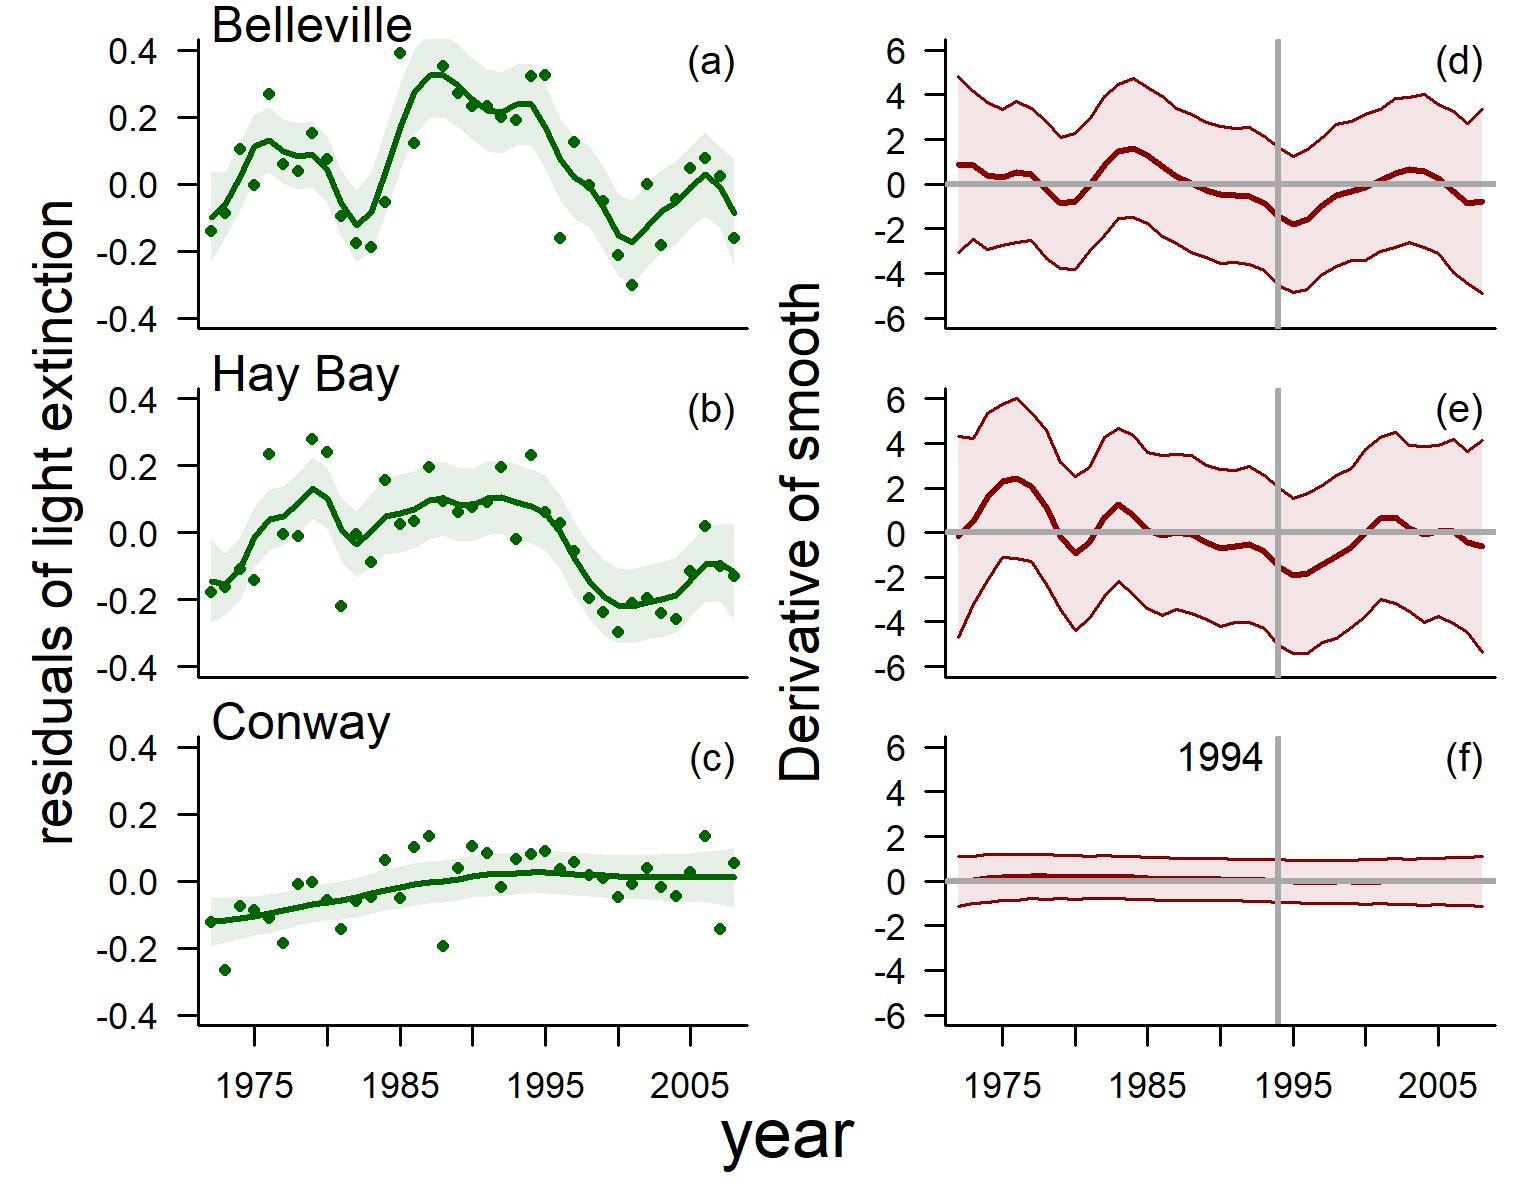
\includegraphics[width=0.7\linewidth]{gamresidlightApr05} \end{center}

\href{}{Currie \& Cuddington, in prep}

`
\end{block}

\begin{block}{Conclusion: Probably just slow change and a small
disturbance}
\protect\hypertarget{conclusion-probably-just-slow-change-and-a-small-disturbance}{}
\begin{itemize}
\tightlist
\item
  however, it could be the system DOES have bistable dynamics but either
\end{itemize}

\begin{enumerate}
\tightlist
\item
  the parameter values are in a regime such that there is no sudden
  change
\item
  the parameter values DO allow sudden change, but there is a long
  transient before that change
\end{enumerate}

\begin{itemize}
\tightlist
\item
  in either case, Zebra mussels only likely to contribute as a small
  scale disturbance
\end{itemize}
\end{block}

\begin{block}{Lessons for using models from the Quinte project}
\protect\hypertarget{lessons-for-using-models-from-the-quinte-project}{}
\begin{enumerate}
\tightlist
\item
  there are all kinds of dynamic behaviours predicted by even very
  simple mechanistic models (e.g., transients can be very long)
\item
  it is going to be tough to determine mechanism in light of this
  variety of behaviour\ldots but we NEED to because of management
  question
\item
  support analysis with a variety of data-driven models at different
  temporal and spatial scales
\end{enumerate}
\end{block}

\begin{block}{Laubmimer}
\protect\hypertarget{laubmimer}{}
\end{block}
\end{frame}

\begin{frame}{can we use physical models to better understand theory?}
\protect\hypertarget{can-we-use-physical-models-to-better-understand-theory}{}
\begin{block}{Prediction based on explanation: Mechanistic models}
\protect\hypertarget{prediction-based-on-explanation-mechanistic-models}{}
-often mathematical, but need not be so.
\end{block}
\end{frame}

\begin{frame}{Case studies in connecting theory and data}
\protect\hypertarget{case-studies-in-connecting-theory-and-data}{}
\begin{block}{Moving from theory to prediction?}
\protect\hypertarget{moving-from-theory-to-prediction}{}
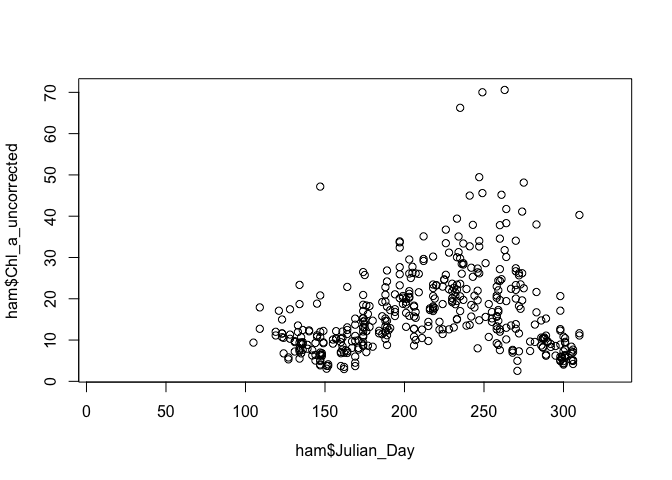
\includegraphics{datatheory_files/figure-beamer/unnamed-chunk-18-1.pdf}
\end{block}

\begin{block}{}
\protect\hypertarget{section-1}{}
Environmental stochasticity or varia- tion in parameter values might
lead to amplification of disturbances {[}24{]} or differences in
expected dynamics. For example, varying parameter values in a
differential equation model can determine whether a monotonic or
oscillating approach to a stable equilibrium is expected (Box 1). There-
fore, uncertainty in parameter values will lead to uncertainty about
which dynamic behaviors are most likely.
\end{block}

\begin{block}{Open Science}
\protect\hypertarget{open-science}{}
\begin{itemize}
\tightlist
\item
  providing data, source code and dynamic documents to make work
  completely reproducible
\item
  Note this document and figures provided at
  \url{https:/github.com/quantitative-biology/talk}
\end{itemize}

\begin{center}\includegraphics[width=0.6\linewidth]{https://imgs.xkcd.com/comics/how_it_works} \end{center}

\url{https://xkcd.com/385/}
\end{block}

\begin{block}{Acknowledgements}
\protect\hypertarget{acknowledgements}{}
We thank Luwen Chang and Matthew Zhou for their amazing learning curves,
and subsequent help coding up the modules. The eCampusOntario grant also
funded several students to evaluate an early version of the materials.
Lina Aragon Baquero, Lauren Banks, Madison Brook, Jacob Burbank, Nicole
Gauvreau and Aranksha Dilip Thakor provided valuable feedback.

The Git and GitHub module builds upon workshop materials that were
originally developed with Chris Grandin (DFO), who AME also thanks for
assistance with the module.
\end{block}

\begin{block}{Funding}
\protect\hypertarget{funding}{}
The Quantitative Biology in Life Science Graduate Programs workshop from
which this work arose which was supported by funding from the Burroughs
Wellcome Fund, from National Science Foundation Award DBI-1300426 for
NIMBioS, with additional support from the University of Tennessee. The
Workshop arose from a partnership between NIMBioS and the Southeast
Center for Mathematics and Biology (SCMB).

Support for the development of online training materials comes from the
Government of Ontario through a grant from eCampusOntario, and the
support of Fisheries and Oceans Canada and the Faculty of Science,
University of Waterloo (\url{https://www.quantitative-biology.ca})
\end{block}

\begin{block}{Other references}
\protect\hypertarget{other-references}{}
Bandura A. 1997. Self-self Efficacy: The Exercise of Control. Freeman,
New York. Charleston L, Leon R. 2016. Constructing self-efficacy in STEM
graduate education. Journal for Multicultural Education 10: 152--166.
Chen Musgrove MM, Schussler EE. 2020. The Ph.D.~panic: examining the
relationships among teaching anxiety, teaching self-efficacy, and coping
in biology graduate teaching assistants (GTAs). bioRxiv DOI
10.1101/2020.02.07.938597. Eaton CD, Highlander HC. 2017. The case for
biocalculus: design, retention, and student performance. CBE---Life
Sciences Education 16: ar25. Flanagan K, Einarson J. 2017. Gender, math
confidence, and grit: relationships with quan- titative skills and
performance in an undergraduate biology course. CBE---Life Sciences
Education 16: ar47. Johnston L, et al.~2019. A graduate student-led
participatory live-coding quantitative methods course in R: experiences
on initiating, developing, and teaching. Journal of Open Source
Education 2: 49. National Research Council et al.~2003. BIO2010:
Transforming undergraduate education for future research biologists.
National Academies Press. Pajares F, Miller MD. 1994. Role of
self-efficacy and self-concept beliefs in mathematical problem solving:
a path analysis. Journal of Educational Psychology 86: 193. Ward-Penny
R, Johnston-Wilder S, Lee C. 2011. Exit interviews: undergraduates who
leave mathematics behind. For the Learning of Mathematics 31: 21--26.
Williams JJ, et al.~2019. Barriers to integration of bioinformatics into
undergraduate life sciences education: a national study of US life
sciences faculty uncover significant barriers to integrating
bioinformatics into undergraduate instruction. PloS one 14: e0224288.
\end{block}

\begin{block}{What do you think?}
\protect\hypertarget{what-do-you-think}{}
\begin{itemize}
\tightlist
\item
  I'm still proofreading
\item
  always want your feedback
  (\url{https://www.quantitative-biology.ca/index.html\#feedback})
\end{itemize}
\end{block}

\begin{block}{Why}
\protect\hypertarget{why}{}
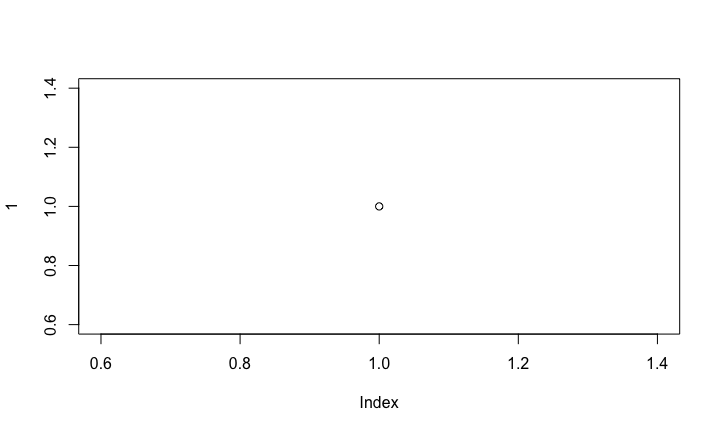
\includegraphics{datatheory_files/figure-beamer/test-1.png}
\end{block}

\begin{block}{Second slide}
\protect\hypertarget{second-slide}{}
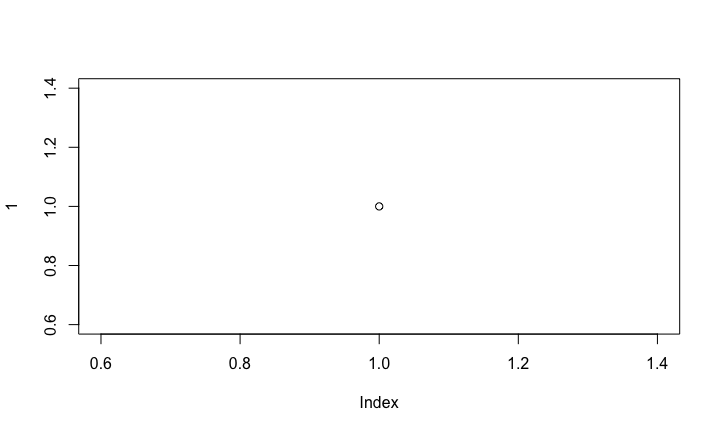
\includegraphics{datatheory_files/figure-beamer/test-1.png}
\end{block}

\begin{block}{}
\protect\hypertarget{section-2}{}
\end{block}
\end{frame}

\end{document}
